\documentclass{article}
\usepackage[utf8]{inputenc}
\usepackage{geometry}
 \geometry{
 a4paper,
 total={170mm,257mm},
 left=20mm,
 top=20mm,
 }
 \usepackage{graphicx}
 \usepackage{titling}
\usepackage{hyperref}
\hypersetup{
    colorlinks=true,
    linkcolor=blue,
    filecolor=magenta,      
    urlcolor=dark,
    pdftitle={Overleaf Example},
    pdfpagemode=FullScreen,
    }

\urlstyle{same}
\usepackage{listings} % Pacote para exibir código fonte
\usepackage{xcolor} % Para colorir a sintaxe do código

\lstset{
  language=SQL,
  basicstyle=\ttfamily\small,
  keywordstyle=\color{blue}\bfseries,
  commentstyle=\color{gray},
  stringstyle=\color{red},
  numbers=left,
  numberstyle=\tiny\color{gray},
  stepnumber=1,
  breaklines=true,
  frame=single
}

 \title{AskSQL}


\author{Cristiano Nicolau}
\date{2025}
 
\usepackage{fancyhdr}


\makeatletter
\def\@maketitle{%
  \newpage
  \null
  \vskip 12em%
  \begin{center}%
  \let \footnote \thanks
    {\Huge \textbf{\@title} \par}%
    \vskip 2em%
    {\LARGE Transforma Linguagem Natural em SQL, Relatórios e Gráficos \par}%
    \vskip 10em%
    {\Large Cristiano Antunes Nicolau \par}%
    \vskip 1em%
    {\Large 108536 \par}%
  \end{center}%
  \par
  \vfill % Push the following content to the bottom of the page
  \begin{center}
      {\large Universidade de Aveiro \par}
    \vskip 0.5em
    {\large Departamento de Electrónica, Telecomunicações e Informática \par}
    \vskip 0.5em
    {\large Mestrado em Ciencia de Dados \par}
    \vskip 0.5em
    {\large Sistemas de Base Dados \par}
    \vskip 0.5em
    \url{https://github.com/cristiano-nicolau/AskSQL}
  \end{center}
  \vskip 2em % Some space before page number
}
\makeatother

\usepackage{lipsum}  
\usepackage{cmbright}

\usepackage{imakeidx}
\makeindex[columns=3, title=Alphabetical Index, intoc]

\begin{document}
\begin{figure}
    \centering
    
\includegraphics[width=0.75\linewidth]{images/deti.png}
    \label{fig:enter-label}
\end{figure}
\maketitle


\clearpage


\tableofcontents
\clearpage

\section{Introdu\c{c}\~ao}


\hspace*{1em} Com o avanço das tecnologias e da inteligência artificial (IA), cada vez mais pessoas procuram realizar tarefas complexas sem a necessidade de conhecimento especializado, recorrendo a aplicações inteligentes que simplificam processos. \\
\hspace*{1em} No contexto da análise de dados, essa tendência tem se refletido na procura por soluções que permitam a qualquer utilizador extrair informações valiosas sem precisar dominar linguagens de programação e/ou ferramentas de BI.
Diante deste cenário, este projeto visa criar uma aplicação que permita que qualquer pessoa, mesmo sem conhecimentos técnicos, consiga criar relatórios e gráficos a partir de consultas em linguagem natural.\\
\hspace*{1em} A ideia principal é proporcionar uma experiência intuitiva ao utilizador, eliminando a necessidade de conhecimento avançado em base de dados ou ferramentas de BI. O utilizador escreve algo como:

\begin{center} "Quero um relatório das vendas por categoria e pais em 2023." \end{center}
\\

A aplicação interpreta o pedido utilizando processamento de linguagem natural (PLN) e, através de um modelo de linguagem de grande escala (LLM), gera automaticamente a query SQL correspondente. Em seguida, a consulta é executada no banco de dados e os dados extraídos são processados e apresentados em relatórios interativos e visualizações dinâmicas, como gráficos de barras, pizza e linhas.

\section{State of the Art}

\hspace*{1em} Nesta secção, vamos abordar alguns trabalhos semelhantes já existentes e explorar as soluções propostas por eles. O objetivo é perceber as abordagens utilizadas, identificar seus pontos fortes e limitações e, com isso, fundamentar as escolhas para o desenvolvimento da nossa solução.\\
\hspace*{1em} Serão analisadas ferramentas que utilizam processamento de linguagem natural para a criação de consultas SQL, bem como sistemas que apresentam relatórios dinâmicos com base em consultas automáticas. Além disso, serão exploradas pesquisas acadêmicas e soluções comerciais que procuram facilitar a interação entre utilizadores não técnicos e base de dados.

\subsection{Graph Maker \cite{graphmaker}}

\hspace*{1em} Este site permite aos utilizadores carregar conjuntos de dados em formatos como CSV e Excel. Com base na query fornecida pelo utilizador, o sistema interpreta a solicitação, agrupa os dados e os organiza conforme as colunas do dataset. A ferramenta visa facilitar a visualização dos dados sem exigir conhecimento técnico avançado, proporcionando gráficos automáticos e personalizáveis conforme as necessidades do usuário. \\
\hspace*{1em} No entanto, sua funcionalidade pode ser limitada quando comparada a soluções que utilizam modelos de linguagem natural para a interpretação de consultas mais complexas.Além disso, o Graph Maker aceita apenas conjuntos de dados provenientes de uma única tabela, não oferecendo suporte a bases de dados relacionais com múltiplas tabelas, o que pode restringir sua aplicabilidade.

\subsection{NL4DV \cite{mitra2022nldv}}

\hspace*{1em} A ferramenta NL4DV (Natural Language for Data Visualization) é uma interface de linguagem natural voltada para a visualização de dados, projetada para permitir que os utilizadores interajam com dados e façam perguntas em linguagem natural, sem a necessidade de conhecimento técnico aprofundado em ferramentas tradicionais de visualização.\\
\hspace*{1em} Os autores do artigo desenvolveram uma biblioteca em Python que recebe uma consulta (query) em linguagem natural junto com o conjunto de dados e gera visualizações apropriadas como resposta. A biblioteca utiliza técnicas de processamento de linguagem natural (NLP) para interpretar a query do utilizador, identifica os tipos de dados e o contexto da solicitação, e em seguida, determinar qual visualização seria a mais adequada. \\
\hspace*{1em} Uma das maiores limitações é que a biblioteca só aceita conjuntos de dados estruturados em formato de tabela, ou seja, como DataFrames em bibliotecas como o pandas, e não permite a integração direta com base de dados relacionais ou outras fontes de dados mais complexas, como bases de dados NoSQL ou dados em tempo real.

\subsection{Text2SQL.AI \cite{text2sql}}

\hspace*{1em} A ferramenta Text2SQL.AI utiliza Processamento de Linguagem Natural (PLN) para converter perguntas feitas em linguagem natural em consultas SQL automaticamente. Isso facilita a análise de dados, permitindo que os utilizadores sem conhecimento avançado em SQL interajam de forma intuitiva com base de dados, sem a necessidade de compreender a sintaxe complexa de SQL. \\
\hspace*{1em} Para avaliar a eficácia da ferramenta, realizei dois testes com diferentes níveis de complexidade de consultas, sem fornecer explicitamente a estrutura da base de dados. A seguir, estão os detalhes dos testes:
\\
\\
1. Teste de consulta simples: \\
Consulta: \textit{'List of all students enrolled in the Database Systems course born in 2003.'}

\begin{lstlisting}
SELECT s.name FROM students s 
JOIN enrollments e ON s.student_id = e.student_id 
JOIN courses c ON e.course_id = c.course_id 
WHERE c.course_name = 'Database Systems' 
AND YEAR(s.birth_date) = 2003; 
\end{lstlisting}

Neste primeiro caso, a ferramenta conseguiu gerar a consulta SQL corretamente, realizando os joins necessários entre as tabelas \texttt{students}, \texttt{enrollments} e \texttt{courses}, e aplicando o filtro adequado para selecionar os estudantes nascidos em 2003. A consulta gerada foi precisa e atendeu à expectativa.
\\
\\
2. Teste de consulta mais complexa:\\
Consulta: \textit{'List the functionaries that have a salary bigger than 1300\$ and work in OPORTO city, and have more than 57 years.'}

\begin{lstlisting}
SELECT name
FROM employees
WHERE salary > 1300
AND city = 'Oporto'
AND age > 57;
\end{lstlisting}

Embora a consulta SQL gerada estivesse sintaticamente correta, ela não retornou o resultado esperado, pois faltava considerar as tabelas adicionais que associam os funcionários às suas respectivas cidades e outras condições relevantes. Isso ocorre porque a consulta não envolveu os joins necessários entre as tabelas, o que resultou em uma resposta incompleta.\\
\hspace*{1em} Após explicar ao chatbot que era necessário realizar joins com outras tabelas para obter as informações corretas, a ferramenta gerou a consulta esperada:

\begin{lstlisting}
SELECT e.name
FROM employees e
JOIN work w ON e.employee_id = w.employee_id
JOIN company c ON w.company_id = c.company_id
WHERE e.salary > 1300
AND c.city = 'Oporto'
AND e.age > 57;
\end{lstlisting}

Desta forma, a ferramenta foi capaz de entender a necessidade de juntar informações das tabelas \texttt{employees}, \texttt{work} e \texttt{company}, gerando a consulta correta que atendeu aos requisitos do enunciado. Isso destaca que, embora o Text2SQL.AI funcione bem em casos simples, ele pode enfrentar desafios em consultas mais complexas, especialmente quando é necessário compreender relações entre múltiplas tabelas.\\
\hspace*{1em} Estes testes demonstram que, para consultas mais complexas, pode ser necessário fornecer um pouco mais de contexto à ferramenta, para que ela possa interpretar corretamente a estrutura do banco de dados e realizar os joins necessários.

\subsection{Spider \cite{spider2025}}

\hspace*{1em} O Spider é um benchmark muito utilizado para a avaliação de modelos Text-to-SQL. Criado pelo grupo YALE LILY, contém um extenso e diversificado conjunto de dados, projetado para avaliar a capacidade de modelos de IA em converter perguntas feitas em linguagem natural para consultas SQL. O Spider abrange uma grande variedade de tópicos, de consultas simples a consultas mais complexas, e inclui uma diversidade de base de dados e esquemas para testar a generalização dos modelos em diferentes contextos de dados. \\
\hspace*{1em} A complexidade do Spider não se limita apenas à variedade das perguntas, mas também à necessidade de o modelo realizar múltiplos joins, subconsultas e manipulações complexas de dados para gerar SQL válido. Essa diversidade torna o Spider um benchmark essencial para o desenvolvimento e avaliação de modelos Text-to-SQL, e é muito utilizado para treinar e testar modelos de machine learning que procuram converter linguagem natural em SQL.\\
\hspace*{1em} Inicialmente, pensei em treinar um modelo de Text-to-SQL a partir do Spider, devido à riqueza do conjunto de dados. No entanto, durante a pesquisa, encontrei alguns modelos já treinados e otimizado utilizando o Spider, falados na subsecção seguinte

\subsection{Modelos Text-to-SQL do Hugging Face \cite{huggingface}}

\hspace*{1em} O Hugging Face oferece uma variedade de modelos Text-to-SQL projetados para converter perguntas feitas em linguagem natural em consultas SQL. Esses modelos, que utilizam arquiteturas avançadas como o T5 (Text-To-Text Transfer Transformer) e outros transformers, são treinados em grandes benchmarks, como o Spider, para fornecer soluções eficazes em conversão de texto para SQL.\\
\hspace*{1em} Estes modelos aproveitam o poder dos transformers para lidar com tarefas de processamento de linguagem natural, como tradução e resposta a perguntas, adaptando essas capacidades para gerar consultas SQL. O T5, por exemplo, é um modelo pré-treinado que pode ser afinado para uma variedade de tarefas de NLP (Natural Language Process), incluindo a conversão de texto para SQL. \\
\hspace*{1em} Estes modelos Text-to-SQL do Hugging Face mostram-se eficazes em tarefas que exigem a criação de consultas SQL de forma automática. Eles são particularmente úteis em cenários onde os utilziadores não têm conhecimento em SQL, mas precisam realizar consultas em base de dados usando apenas linguagem natural.

\subsection{ChatGPT \cite{chatgpt2025}}

\hspace*{1em} Como parte da pesquisa, também realizei os mesmos testes de consultas SQL utilizando o ChatGPT. Para isso, forneci ao modelo a descrição das tabelas da base de dados e as questões a serem resolvidas. O objetivo era testar a capacidade do modelo em gerar consultas SQL corretamente a partir de linguagem natural, considerando a estrutura do banco de dados fornecida.

\begin{lstlisting} 
Transforma a seguinte frase numa querie SQL:
"Quero todos os alunos nascidos em 2003 inscritos na uc Sistemas de Base Dados"

Tenho o seguinte schema:
Alunos -  nmec, nome, ano_nascimento
incricoes- nmec, id_disciplina
uc - id, nome, nr_maximo_inscritos
\end{lstlisting}

O ChatGPT gerou a seguinte consulta SQL, que foi capaz de fornecer o resultado esperado:

\begin{lstlisting} 
SELECT a.nmec, a.nome, a.ano_nascimento 
FROM Alunos a 
JOIN inscricoes i ON a.nmec = i.nmec 
JOIN uc u ON i.id_disciplina = u.id 
WHERE a.ano_nascimento = 2003 
AND u.nome = 'Sistemas de Base de Dados'; 
\end{lstlisting}

A consulta gerada foi precisa e atendeu às expectativas. O modelo foi capaz de realizar corretamente os joins entre as tabelas \texttt{alunos}, \texttt{inscrições} e \texttt{uc} , aplicando os filtros necessários para selecionar os alunos nascidos em 2003 e inscritos na unidade curricular "Sistemas de Base de Dados".vApós obter esses resultados com o ChatGPT, comecei o desenvolvimento da aplicação.

\section{Metodologia}

\hspace*{1em} Nesta secção retrato a metodologia utilizada ao longo do projeto. A metodologia foi dividida em três partes principais, com o objetivo de explorar diferentes abordagens para lidar com consultas SQL a partir de linguagem natural: a primeira foca em trabalhar com datasets simples (compostos por uma única tabela), a segunda aborda bases de dados mais complexas com múltiplas tabelas, e a terceira trata da visualização dos dados em uma interface interativa. Essa divisão permite testar diferentes estratégias e avaliar as limitações dos modelos em cenários distintos.

\subsection{Parte 1: Experimentar modelos NLP para quando recebo datasets de uma tabela} 

\hspace*{1em} O primeiro desafio consiste em trabalhar com datasets compostos por uma única tabela. Com este cenário, o meu objetivo é através de modelos de Processamento de Linguagem Natural (NLP) ser capaz de compreender consultas feitas em linguagem natural e traduzi-las em consultas SQL válidas. 

 Como o modelo lida apenas com uma tabela, a complexidade é menor, já que não será necessário realizar joins com outras tabelas, mas sim focar em uma tradução direta da linguagem natural para a sintaxe SQL, considerando as colunas dessa única tabela.

\subsection{Parte 2: Trabalhar com modelos Text-to-SQL para conexões com base de dados de múltiplas tabelas} 

\hspace*{1em} A segunda parte da metodologia envolve trabalhar com base de dados que possuem múltiplas tabelas, o que traz desafios adicionais, como a necessidade de realizar joins, aplicar múltiplas condições WHERE, e lidar com relações complexas entre as tabelas.\\ \hspace*{1em} Para esta parte, pretendo explorar modelos Text-to-SQL já existentes, com o objetivo de gerar consultas SQL a partir de linguagem natural, considerando a estrutura e os relacionamentos entre as diversas tabelas da base de dados. Aqui, a abordagem será testar diferentes modelos para entender como eles lidam com esses casos mais complexos e onde as suas limitações podem surgir.

Esta divisão da metodologia procurar explorar as vantagens e desafios de cada tipo de dado (dataset simples vs. base de dados complexa) e permitirá uma análise detalhada das soluções que podem ser aplicadas para cada cenário.

\subsection{Parte 3: Visualização dos dados em uma interface interativa} 

\hspace*{1em} Após a conversão das consultas para SQL e a extração dos dados, a terceira parte da metodologia concentra-se na visualização dos resultados em uma interface web interativa.

A interface deve ser intuitiva e eficiente, permitindo que os utilizadores insiram consultas em linguagem natural e visualizem os resultados de forma clara. Além disso, para facilitar a análise dos dados, a aplicação deve incluir funcionalidades como:

\begin{enumerate}
    \item \textbf{Geração de gráficos interativos} para representar visualmente as informações extraídas da base de dados.
    \item \textbf{Criação de relatórios} estruturados para que os utilizadores possam obter insights detalhados a partir das consultas realizadas.
\end{enumerate}

Com esta abordagem, procuramos uma solução completa que, através da geração de queries SQL, torne a análise de dados mais acessível e eficiente, com uma melhor experiência de utilizador, principalmente para pessoas sem conhecimentos técnicos.


\section{Modelo Text to SQL}

\hspace*{1em} Nesta seção, explico o caminho seguido no desenvolvimento do meu projeto. A implementação foi dividida em duas partes distintas, com base no tipo de dados com os quais os modelos seriam testados:

\begin{itemize}
    \item \textbf{Parte 1:} Criação de um algoritmo NLP próprio ou a utilização de modelos existentes para lidar com datasets contendo apenas uma única tabela. O objetivo aqui foi desenvolver um modelo que fosse capaz de gerar consultas SQL a partir de uma linguagem natural simples, sem a necessidade de realizar joins ou interagir com múltiplas tabelas.
    \item \textbf{Parte 2:} Uso de modelos Text-to-SQL para transformar consultas em linguagem natural em SQL, focando em bancos de dados com múltiplas tabelas. O propósito nesta segunda parte foi avaliar como diferentes modelos lidariam com consultas SQL mais complexas, que exigem a combinação de múltiplas tabelas e a aplicação de condições diversas.
\end{itemize}

A ideia é analisar como cada abordagem e modelo se comporta, desde consultas SQL simples até aquelas que exijam maior complexidade, como múltiplos joins e filtros avançados.

A ideia inicial seria dividir em duas partes, mas optei por não dividir esta secção em duas partes, uma vez que ao fazer a investigação para a segunda parte, para as tabelas mais complexas, realizei testes mais simples com casos de uma tabela só. \\
\hspace*{1em} Na Parte 2 do projeto, o foco foi lidar com bases de dados que envolvem múltiplas tabelas, onde as consultas SQL se tornam mais complexas, exigindo a utilização de joins e múltiplas condições. Para isso, testei diversos modelos Text-to-SQL com o objetivo de avaliar como cada um lida com essas consultas mais complexas.

 \subsection{T5-Base-Text-to-SQL} 
\hspace*{1em}Primeiramente, comecei por utilizar o modelo T5-Base-Text-to-SQL do Hugging Face, criado por suriya7 \cite{raffel2019exploring}, um modelo amplamente utilizado na conversão de consultas em linguagem natural para SQL. No entanto, durante os testes, não consegui obter resultados. O modelo não foi capaz de gerar as consultas SQL para os cenários apresentados, sugerindo limitações no contexto de consultas mais complexas envolvendo múltiplas tabelas. 

\subsection{t5-small-awesome-text-to-sql} 
\hspace*{1em} Na sequência, testei o modelo cssupport/t5-small-awesome-text-to-sql \cite{cssupport_t5small2025}. Este modelo teve um melhor desempenho, sendo eficaz na criação de tabelas e na inserção de dados. No entanto, ao tentar gerar consultas SQL do tipo SELECT, o modelo não foi capaz de o fazer, visto que foi criado só e apenas para a criação e inserção de dados SQL.

\subsection{text-to-sql-with-table-schema} 
\hspace*{1em} Em seguida, explorei o modelo juierror/text-to-sql-with-table-schema \cite{juierror2025}. Este modelo mostrou um bom desempenho, funcionando bem para gerar consultas SQL a partir de um único conjunto de dados com várias colunas. No entanto, quando as consultas se tornaram mais complexas, com múltiplos joins ou condições WHERE, o modelo não foi capaz de gerar as consultas corretas, devido ao modelo não conseguir lidar com consultas com várias tabelas.


\subsection{flan-t5-text2sql-with-schema-v2} 
\hspace*{1em} Considerando as limitações encontradas, decidi testar a versão atualizada do modelo do mesmo autor: juierror/flan-t5-text2sql-with-schema-v2 \cite{juierror2025flan}. Esta versão foi mais eficaz ao lidar com consultas SQL mais simples, mas ainda assim apresentou falhas em consultas mais complexas que exigiam múltiplos joins e condições avançadas WHERE. Embora tivesse melhor desempenho do que as versões anteriores, em três testes mais complicados, o modelo falhou em gerar o SQL correto. 
\\
\\
Teste 1:
\begin{lstlisting}
Consulta: "List all students who are subscribed in the Database Systems and are born in 2003."

Estrutura das tabelas:
{
    'Students': ['student_id', 'name', 'birth_year'],
    'Courses': ['course_id', 'name', 'max_enrollments'],
    'Enrollments': ['student_id', 'course_id']
}

Consulta SQL gerada:
SELECT T1.name 
FROM students AS T1 
JOIN enrollments AS T2 ON T1.student_id = T2.student_id 
WHERE T2.course_id = 'Database Systems' 
AND T1.birth_year = 2003
\end{lstlisting}

O código SQL gerado apresentou um erro importante no filtro do nome do curso. A consulta tenta comparar o course\_id com o nome do curso diretamente, mas o course\_id é um identificador numérico enquanto o nome do curso ("Database Systems") está presente na tabela Courses, e não em Enrollments.
\\
\\
Teste 2:

\begin{lstlisting}
Consulta: "List names of employees who have a salary greater than $1300, work in the city of Oporto and are younger than 30 years."

Estrutura das tabelas:
{ 
    'employees': ['employee_id', 'name', 'salary', 'age'],
    'company': ['company_id', 'name', 'city'], 
    'work': ['employee_id', 'company_id']
}

Consulta SQL gerada:
SELECT t1.name 
FROM employees AS t1 
JOIN work AS t2 ON t1.employee_id = t2.employee_id 
JOIN company AS t3 ON t2.company_id = t3.company_id 
WHERE t3.city = 'Oporto' 
AND t1.age < 30
\end{lstlisting}

A consulta SQL gerada está quase correta, mas faltou a condição para filtrar os funcionários com salário superior a \$1300. Este erro mostrou mais uma vez que este modelo tem algumas falhas, impossibilitando o uso do mesmo na minha aplicação.
\\
\\

\subsection{Groq - Llama-3.3-70b-versatile}
\hspace*{1em} Dado que os modelos mencionados apresentaram limitações nas consultas mais complexas, decidi explorar uma abordagem mais avançada. Pesquisando por modelos LLMs, optei por usar o modelo Llama-3.3-70b-versatile da Groq \cite{groq2025}.

A Groq é uma plataforma que oferece aceleração de hardware e software para execução de modelos de inteligência artificial, permitindo um processamento mais rápido e eficiente. O modelo Llama-3.3-70b-versatile é um modelo de linguagem natural desenvolvido pela Meta, com 70 bilhões de parâmetros, o que lhe confere uma boa capacidade de lidar com uma variedade de tarefas, incluindo a conversão de linguagem natural em SQL.

Ao fornecer o schema da base de dados, consegui facilmente obter os resultados esperados, mesmo para consultas mais complexas que exigiam múltiplos joins e condições avançadas WHERE. Esta abordagem superou as limitações dos modelos anteriores, garantindo maior eficiência na extração de dados.
\\
Teste Realizado:


\begin{itemize}
    \item \textbf{Query 1:} 'List all students who are subscribed in the Database Systems and are born in 2003.'
    \item \textbf{Query 2:} 'List names of employees who have a salary greater than \$1300, work in the city of Oporto and are younger than 30 years.'
\end{itemize}
Estrutura das tabelas:
\begin{lstlisting}
{
    'teste1.Students': ['student_id', 'name', 'birth_year'],
    'teste1.Courses': ['course_id', 'name', 'max_enrollments'],
    'teste1.Enrollments': ['student_id', 'course_id'], 
    
    'test2.employees': ['employee_id', 'name', 'salary', 'age'],
    'test2.company': ['company_id', 'name', 'city'], 
    'test2.work': ['employee_id', 'company_id']
}
\end{lstlisting}
\\
Query 1 gerada:
\begin{lstlisting}
SELECT S.name
FROM teste1.Students S
JOIN teste1.Enrollments E ON S.student_id = E.student_id
JOIN teste1.Courses C ON E.course_id = C.course_id
WHERE C.name = 'Database Systems' AND S.birth_year = 2003;
\end{lstlisting}
\\
Query 2 gerada:
\begin{lstlisting}
SELECT E.name
FROM test2.employees E
JOIN test2.work W ON E.employee_id = W.employee_id
JOIN test2.company C ON W.company_id = C.company_id
WHERE E.salary > 1300 AND C.city = 'Oporto' AND E.age < 30;
\end{lstlisting}

O Llama-3.3-70B-Versatile demonstrou excelente desempenho ao interpretar a estrutura da base de dados e gerar consultas SQL corretas e bem otimizadas. Mesmo em cenários que exijam múltiplos joins e filtros complexos, o modelo conseguiu entregar as respostas corretas e esperadas. Dado o seu alto nível de precisão e eficiência na conversão de linguagem natural em SQL, este modelo foi o escolhido como solução para a aplicação. Com isso, os utilizadores, independentemente do seu conhecimento técnico em base de dados, conseguem aceder e visualizar facilmente as informações desejadas.

\section{Implementação}

\hspace*{1em} Nesta seção, descrevo a implementação do modelo escolhido no capítulo anterior, bem como as decisões tomadas em relação à interface e ao funcionamento da aplicação.


\subsection{Interface}
\hspace*{1em} Após a seleção de um modelo eficiente para a transformação das queries em texto para SQL, é necessário o desenvolvimento de uma interface intuitiva e funcional. Para isso, optei pelo Streamlit, uma tecnologia que se destaca pela sua simplicidade, flexibilidade e facilidade na criação de aplicações web interativas com pouco código.

O Streamlit permite uma integração ágil com modelos de IA e bases de dados, tornando-o uma solução ideal para este projeto. Além disso, sua interface dinâmica proporciona uma experiência de utilizador fluida, facilitando a inserção de consultas em linguagem natural e a visualização dos resultados em tempo real.


\subsection{Funcionalidades da Aplicação}
A aplicação desenvolvida consiste em um chatbot com três funcionalidades principais:

\begin{itemize}
    \item \textbf{Geração de Relatórios} – Criação automatizada de relatórios estruturados com base nos dados fornecidos, permitindo uma análise detalhada e organizada das informações extraídas.
    \item \textbf{Geração de Gráficos} – Visualização interativa dos dados por meio de gráficos dinâmicos, facilitando a interpretação e identificação de padrões nos resultados.
    \item \textbf{Construção de Consultas SQL }– Chat que não apenas gera consultas SQL a partir de linguagem natural, mas também explica a estrutura da query criada, auxiliando o utilizador a compreender melhor o processo e os resultados obtidos.
\end{itemize}

Essas funcionalidades trabalham em conjunto para oferecer uma experiência intuitiva, permitindo que utilizadores, independentemente do seu conhecimento técnico, consigam explorar e visualizar os dados de maneira eficiente.

\subsection{Estrutura do Chatbot}

\hspace*{1em} A primeira etapa da aplicação consiste na conexão com a base de dados. Para esta implementação, os detalhes de conexão são passados como parâmetros, pois estamos a utilizar  uma base de dados específica. No entanto, para permitir uma maior generalização, o sistema pode ser configurado para que o utilizador forneça suas credenciais de acesso e o token necessário para interagir com o modelo da Groq.

Cada funcionalidade do chatbot foi desenvolvida de forma modular, permitindo ao utilizador escolher entre os três tipos de interação disponíveis. O sistema interpreta as solicitações e executa as ações correspondentes, seja gerando relatórios, criando visualizações gráficas ou construindo consultas SQL personalizadas.


\subsubsection{Geração de Relatórios}

\hspace*{1em} A funcionalidade de Geração de Relatórios permite que o utilizador obtenha relatórios estruturados com base nos dados disponíveis na base de dados. O processo segue os seguintes passos:

\begin{enumerate}
    \item O utilizador insere um prompt descrevendo o relatório desejado.
    \item A aplicação envia o prompt, juntamente com a estrutura da base de dados, ao modelo da Groq.
    \item O modelo gera uma query SQL correspondente à solicitação do utilizador.
    \item A aplicação executa a consulta na base de dados e recupera os dados resultantes.
    \item Os dados são transformados em um DataFrame para facilitar a visualização e interpretação.
    \item O relatório gerado é apresentado ao utilizador.
\end{enumerate}

Esta abordagem automatiza o processo de criação de relatórios, tornando a análise de dados mais acessível e eficiente.


\subsubsection{Geração de Gráficos}
\hspace*{1em} A funcionalidade de Geração de Gráficos segue um fluxo semelhante à geração de relatórios, mas com um foco na visualização dos dados. O processo é o seguinte:

\begin{enumerate}
    \item O utilizador insere uma pergunta ou solicitação para gerar um gráfico.
    \item A aplicação passa o prompt e a estrutura da base de dados ao modelo da Groq.
    \item O modelo retorna uma query SQL, que é então executada na base de dados.
    \item Os resultados são transformados em um DataFrame.
    \item O DataFrame é enviado novamente ao modelo da Groq, solicitando a geração do código necessário para criar um gráfico utilizando Plotly.
    \item O gráfico é gerado e apresentado na interface.
\end{enumerate}

Esta abordagem permite que utilizadores criem visualizações de dados sem necessidade de conhecimento prévio em SQL ou Plotly, tornando a análise mais intuitiva.


\subsubsection{Construção de Consultas SQL}

\hspace*{1em} A funcionalidade de Construção de Consultas SQL tem como objetivo facilitar a criação e interpretação de consultas SQL. O processo segue os seguintes passos:

\begin{enumerate}
    \item O utilizador insere um prompt descrevendo a informação que deseja obter da base de dados.
    \item A aplicação envia o prompt ao modelo da Groq, que retorna:
    \item A explicação da consulta SQL gerada, detalhando sua estrutura e propósito.
    \item A interface exibe tanto a explicação quanto a consulta SQL, permitindo ao utilizador compreender e, se necessário, modificar a query antes da execução.
\end{enumerate}

Essa funcionalidade é útil para quem deseja aprender SQL, validar consultas antes da execução ou simplesmente obter consultas otimizadas sem esforço manual.

\begin{figure}[!ht]
    \centering
    \textbf{Exemplos das Interfaces} \\[0.3cm] % Adiciona espaço abaixo do título

    \begin{minipage}{0.3\linewidth}
        \centering
        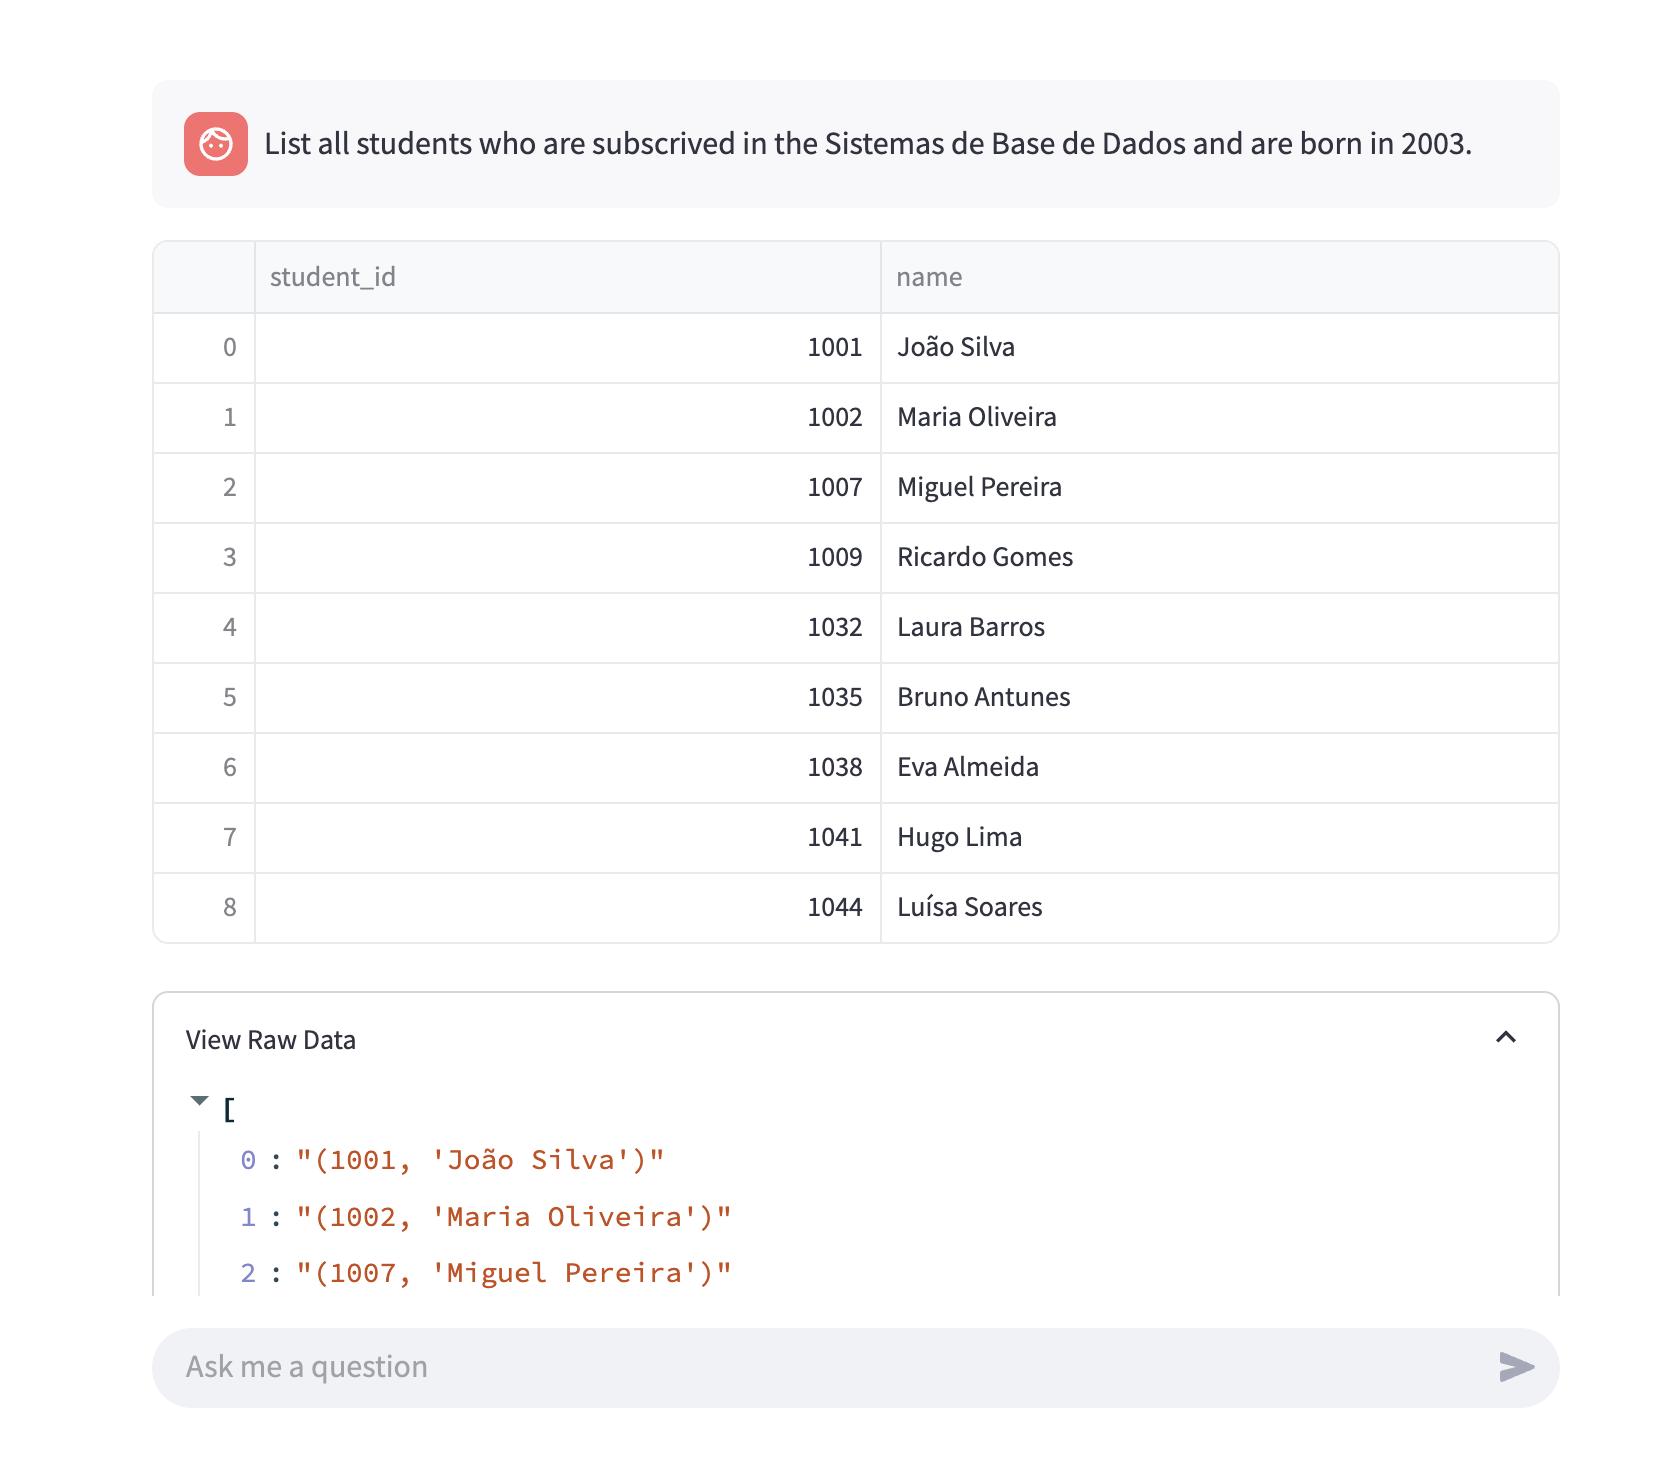
\includegraphics[width=\linewidth]
        {images/report_generator1.png}
        \caption{Exemplo Report Generator}
    \end{minipage}
    \hspace{0.01\linewidth} % Espaço entre as imagens
        \begin{minipage}{0.3\linewidth}
        \centering
        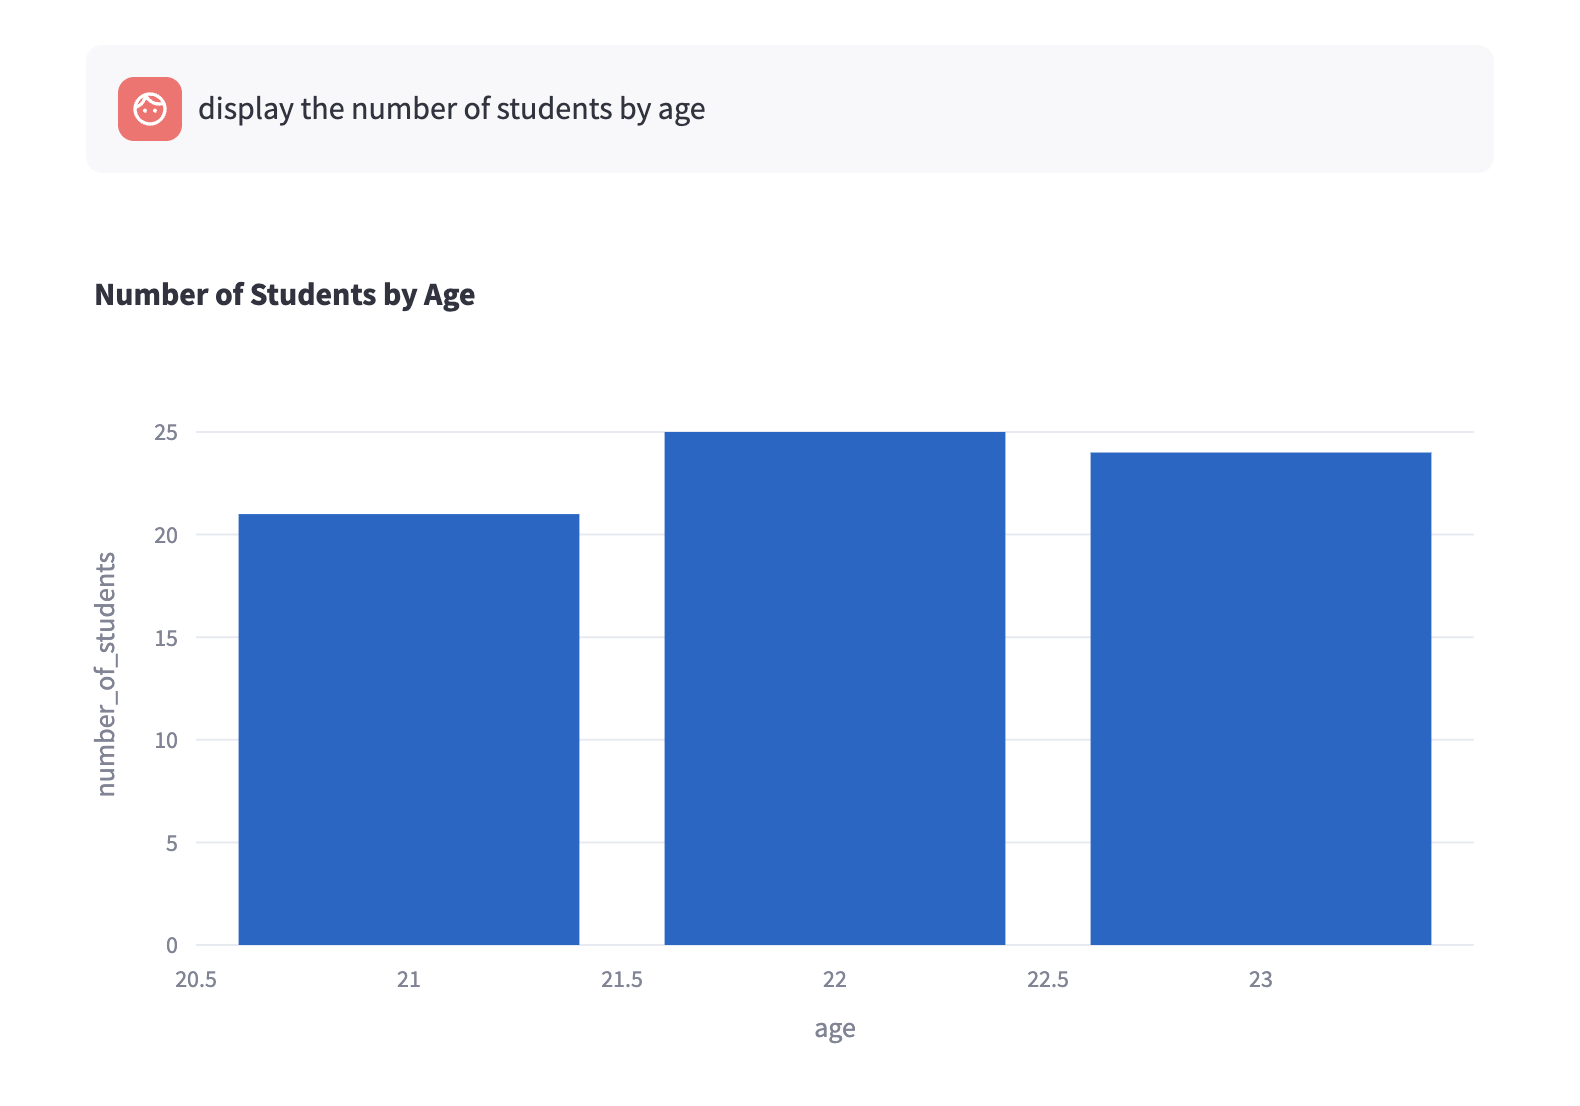
\includegraphics[width=\linewidth]
        {images/chart2.png}
        \caption{Exemplo Chart Generator}
    \end{minipage}
    \hspace{0.01\linewidth} % Espaço entre as imagens
    \begin{minipage}{0.3\linewidth}
        \centering
        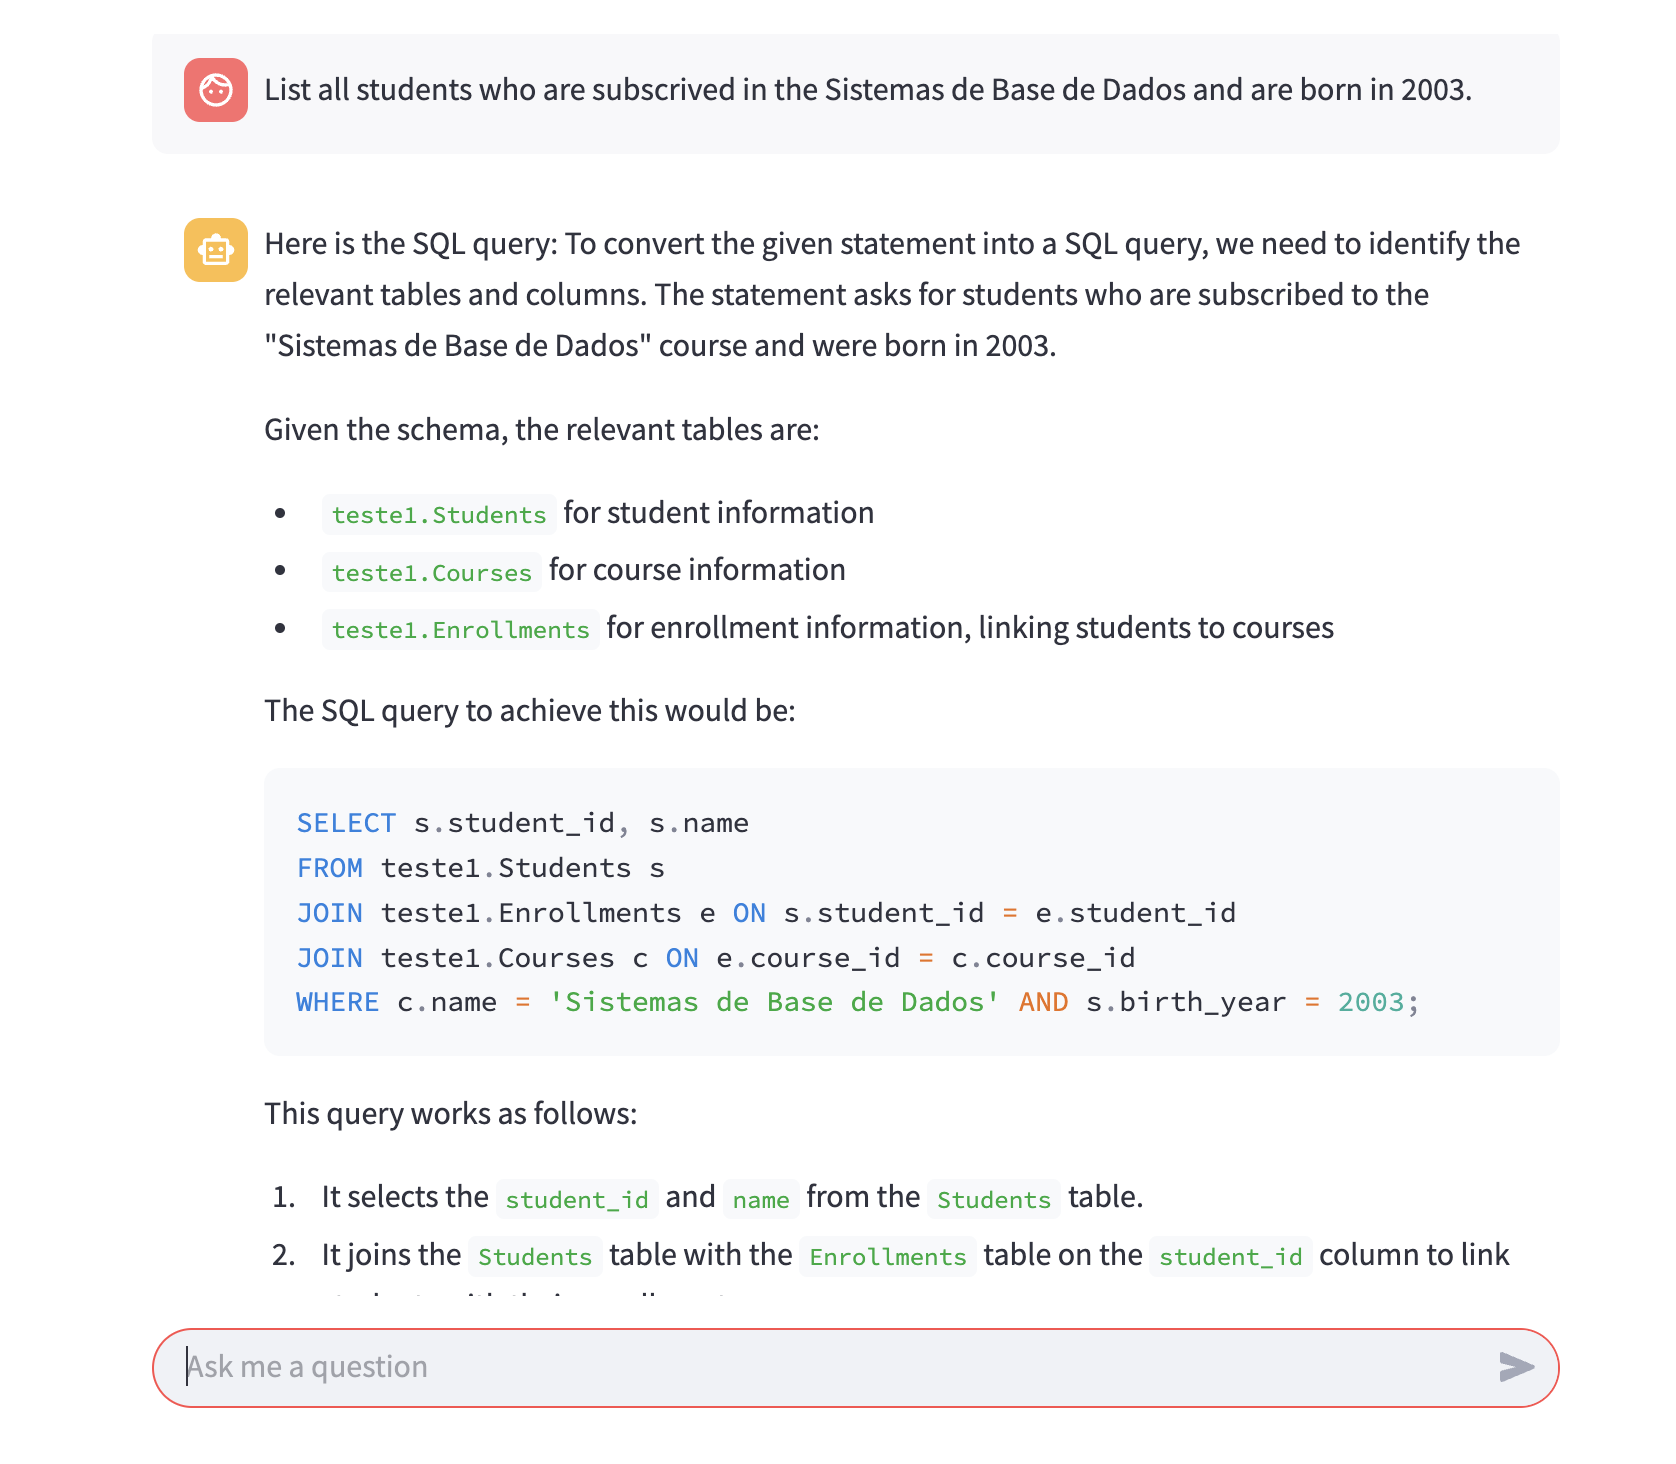
\includegraphics[width=\linewidth]
        {images/sql_generator1.png}
        \caption{Exemplo SQL Generator}
    \end{minipage}
\end{figure}

\subsection{Comandos Adicionais}


\begin{figure}[!h]
    \centering
        \textbf{Exemplos dos comandos adicionais} \\[0.3cm] % Adiciona espaço abaixo do título
    \begin{minipage}{0.46\linewidth}
        \centering
        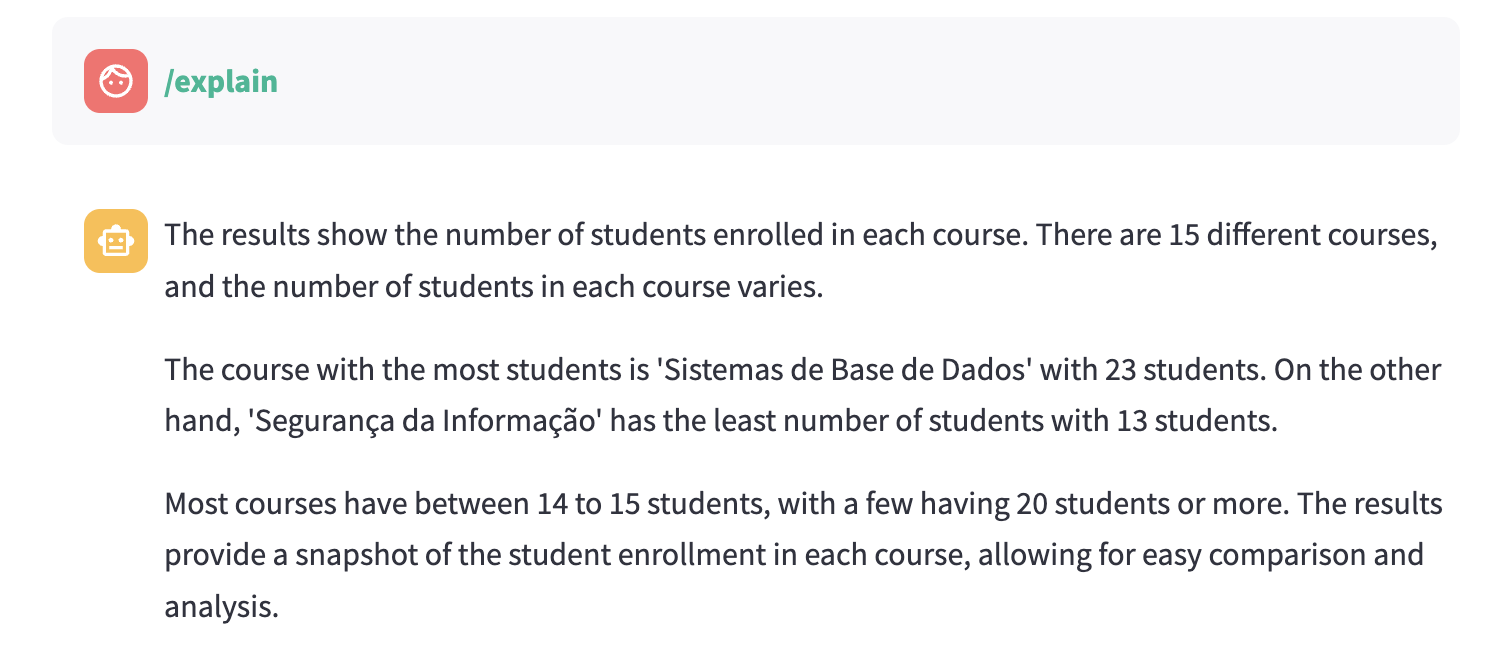
\includegraphics[width=\linewidth]{images/explain.png}
        \caption{Exemplo do comando /explain}
        \label{fig:explain}
    \end{minipage}
    \hspace{0.01\linewidth} % Espaço entre as imagens
    \begin{minipage}{0.46\linewidth}
        \centering
        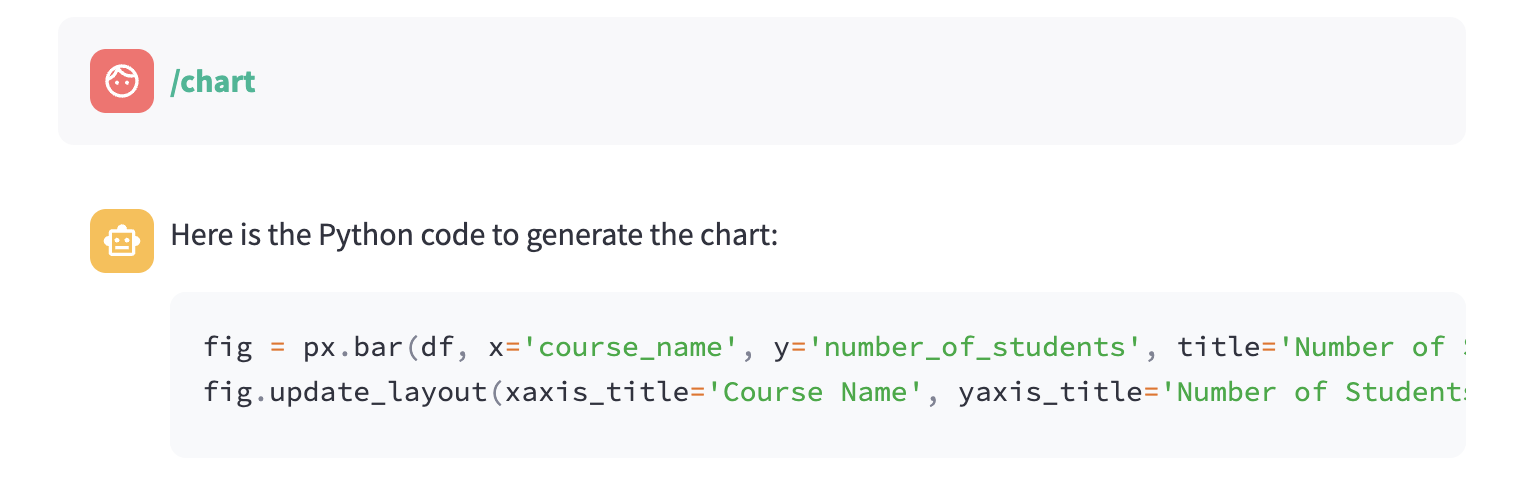
\includegraphics[width=\linewidth]{images/chart.png}
        \caption{Exemplo do comando /chart}
        \label{fig:chart}
    \end{minipage}

    \vspace{0.5cm} % Espaço vertical entre as linhas de imagens

    \begin{minipage}{0.46\linewidth}
        \centering
        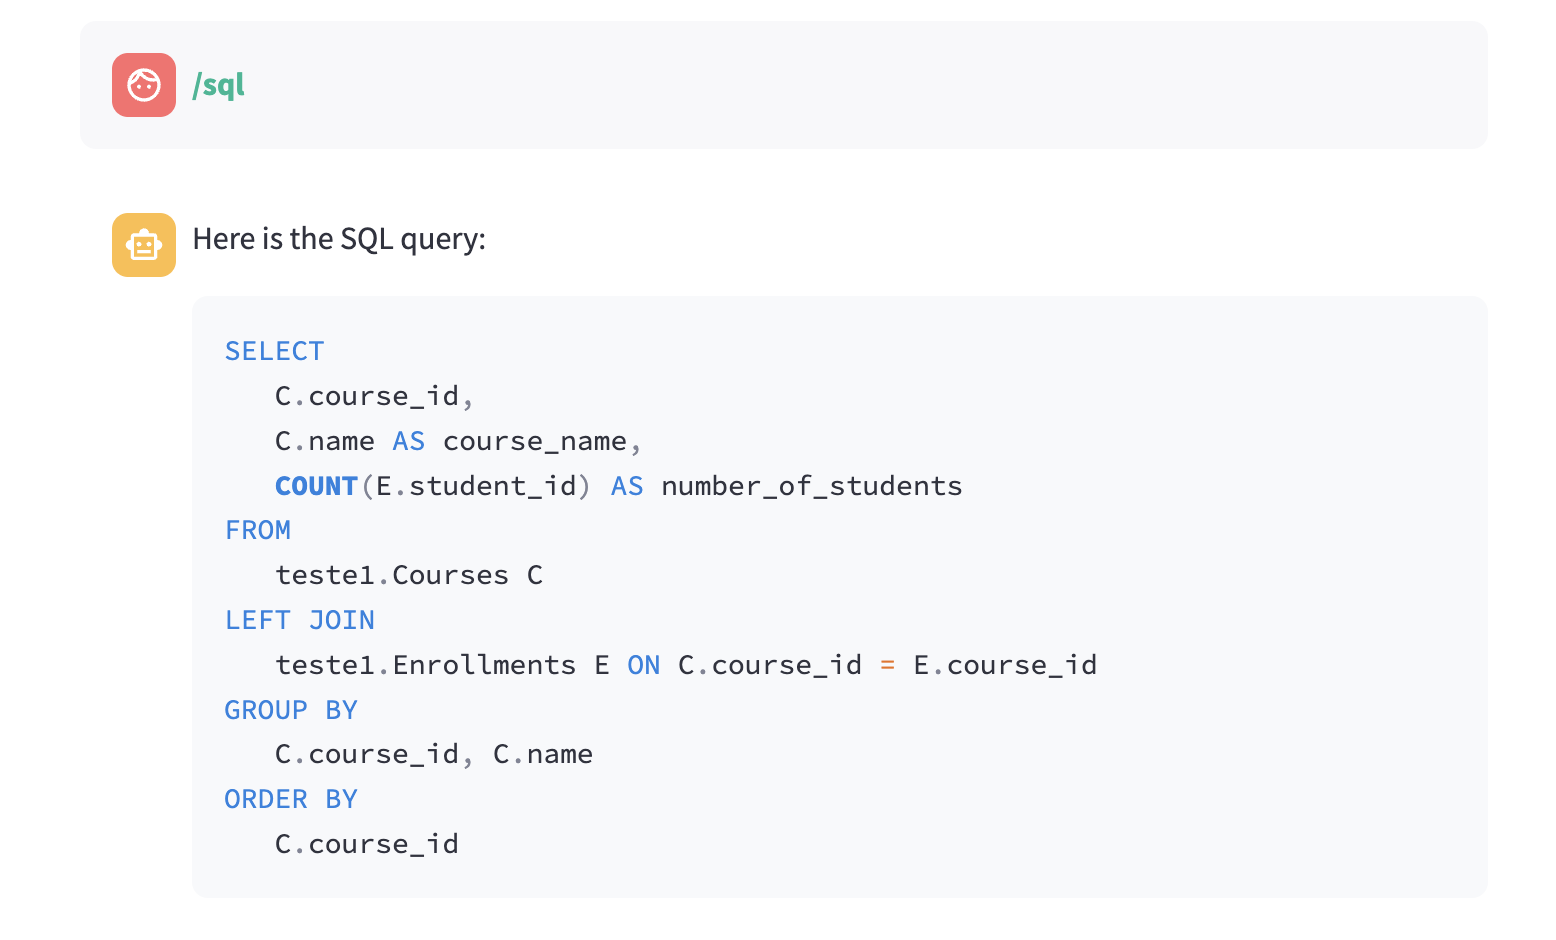
\includegraphics[width=\linewidth]{images/sql.png}
        \caption{Exemplo do comando /sql}
        \label{fig:sql}
    \end{minipage}
    \hspace{0.01\linewidth} % Espaço entre as imagens
    \begin{minipage}{0.46\linewidth}
        \centering
        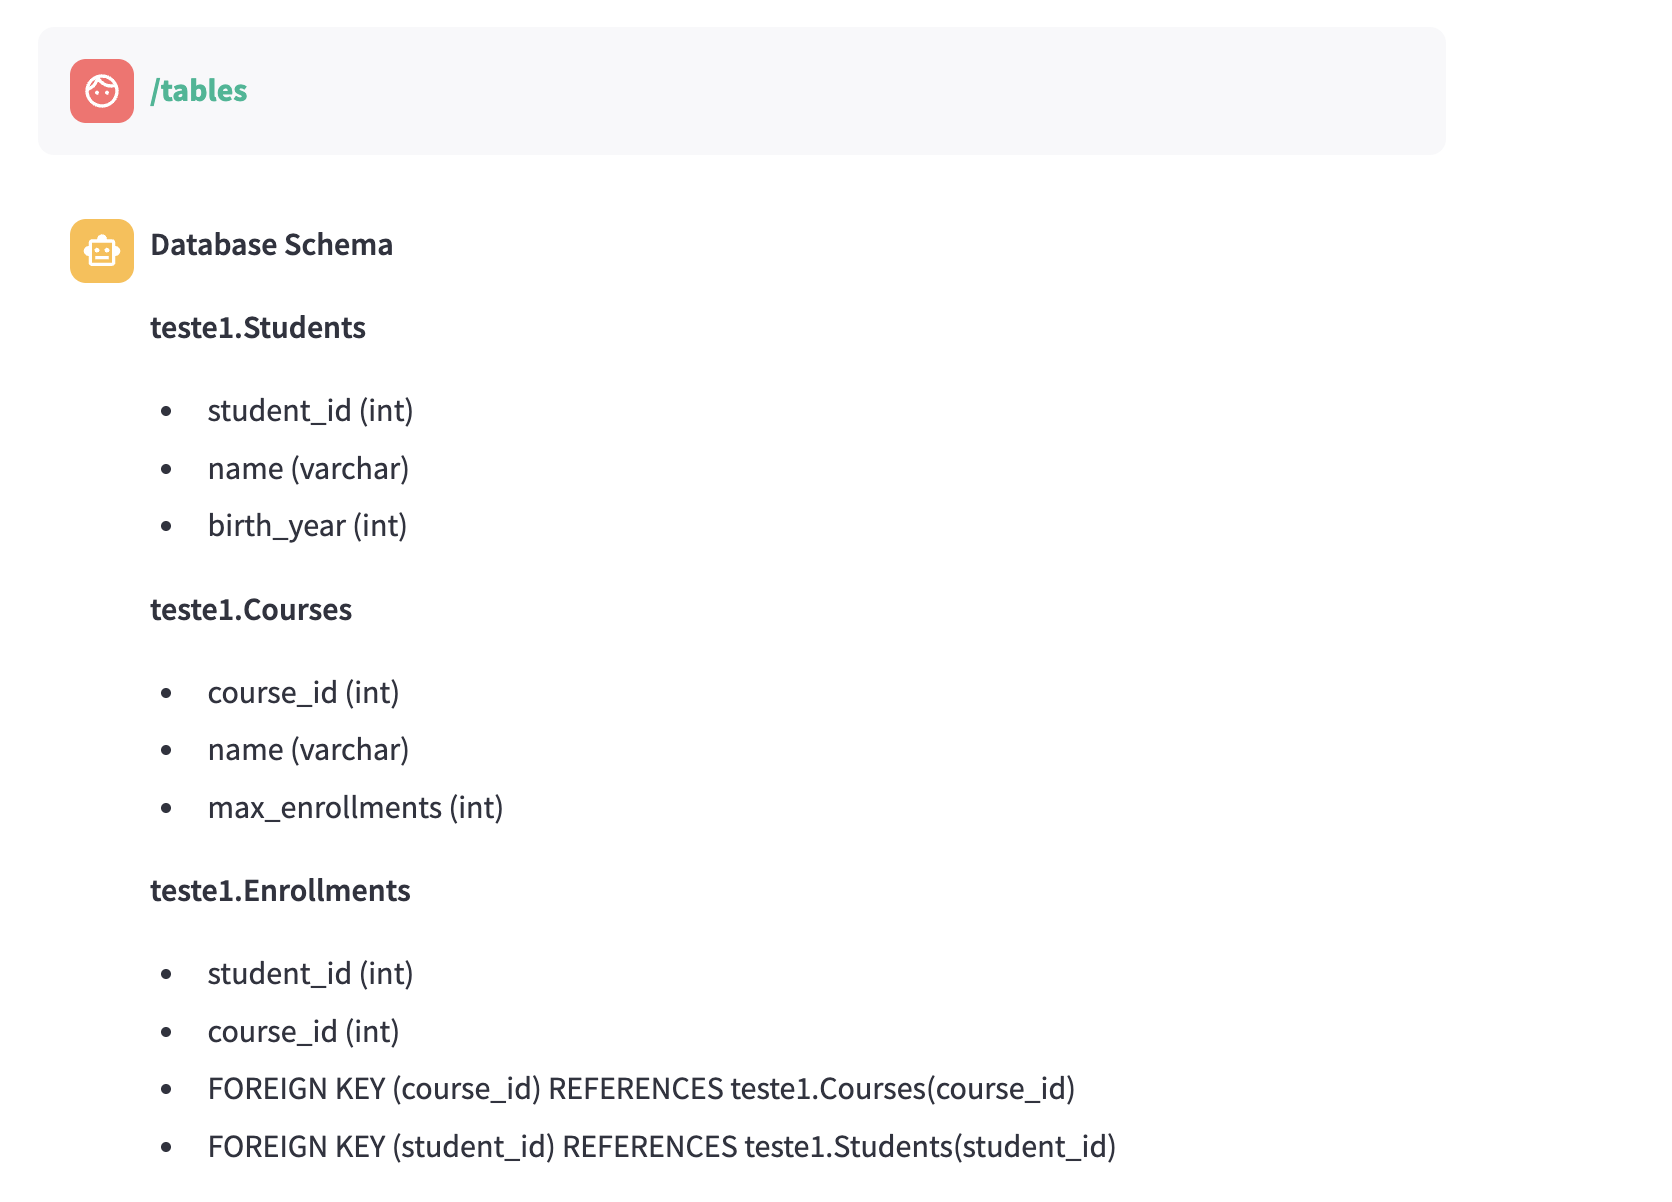
\includegraphics[width=\linewidth]{images/tables.png}
        \caption{Exemplo do comando /tables}
        \label{fig:tables}
    \end{minipage}

        \vspace{0.5cm} % Espaço vertical entre as linhas de imagens

    \begin{minipage}{0.46\linewidth}
        \centering
        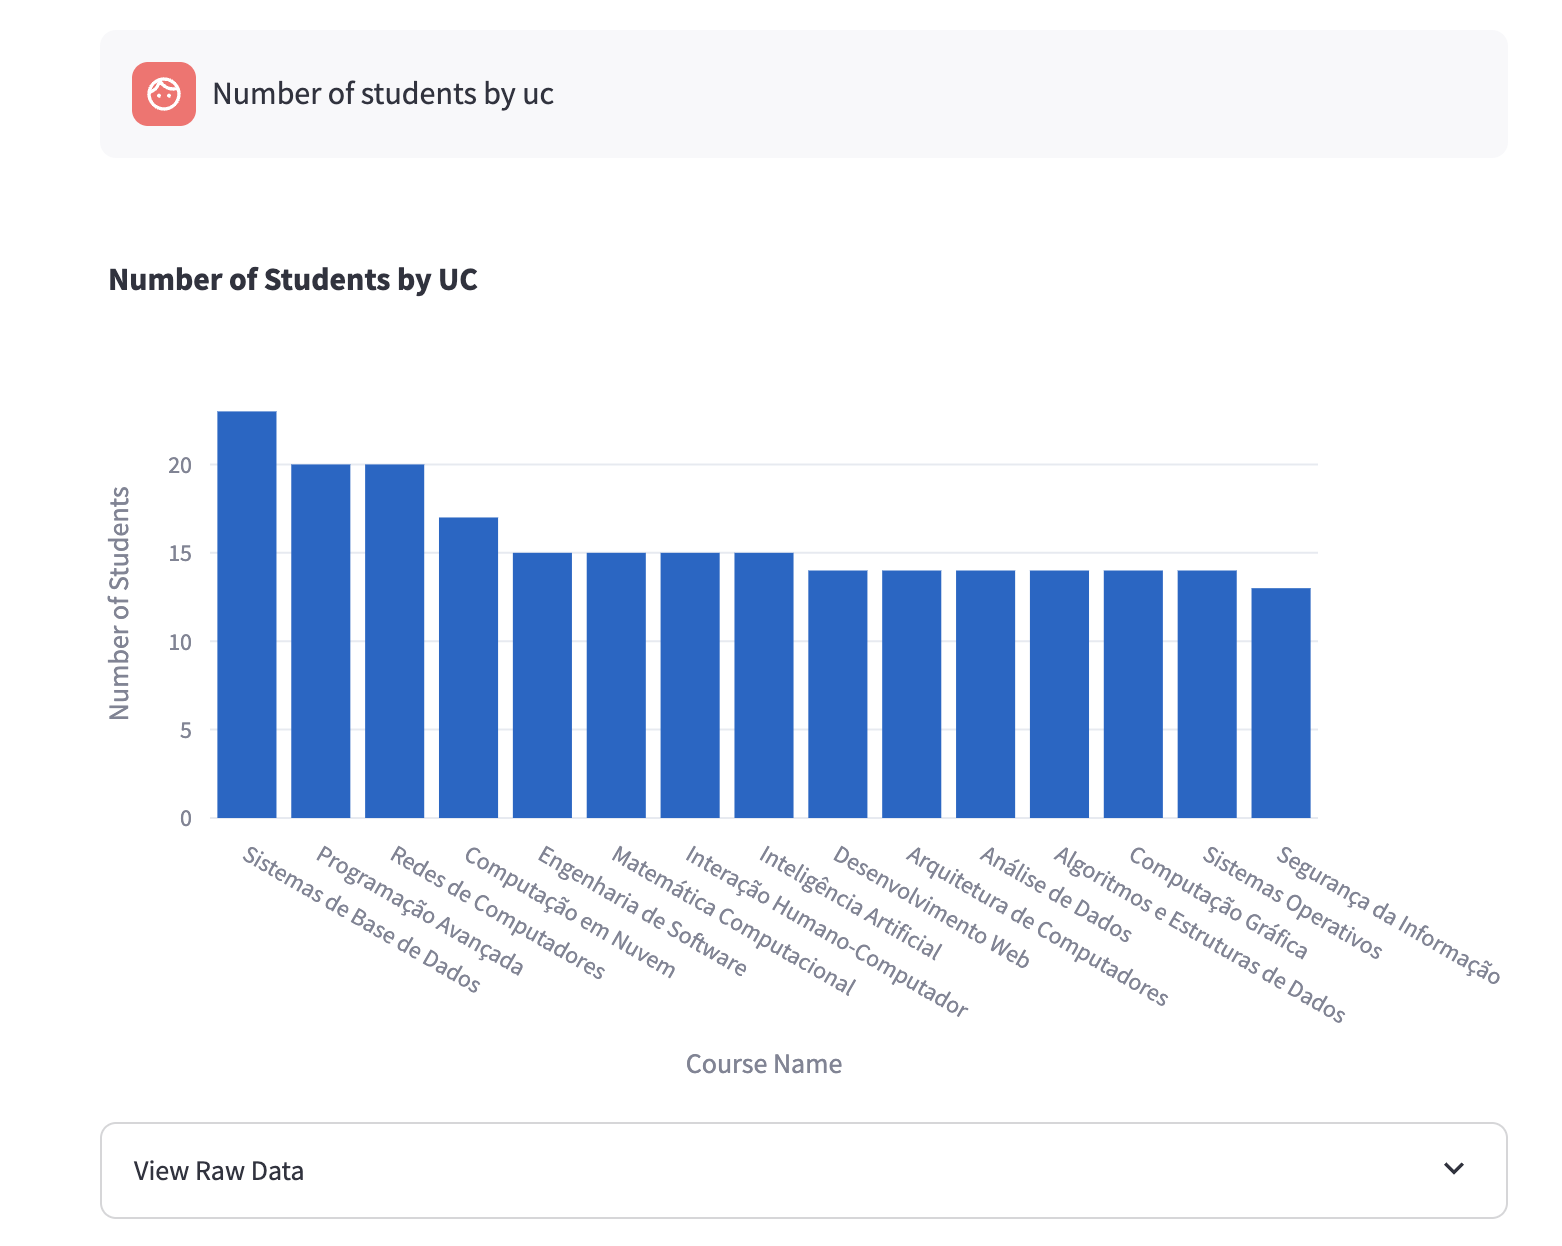
\includegraphics[width=\linewidth]{images/:refactor0.png}
        \caption{Exemplo do comando /refactor}
        \label{fig:sql}
    \end{minipage}
    \hspace{0.01\linewidth} % Espaço entre as imagens
    \begin{minipage}{0.46\linewidth}
        \centering
        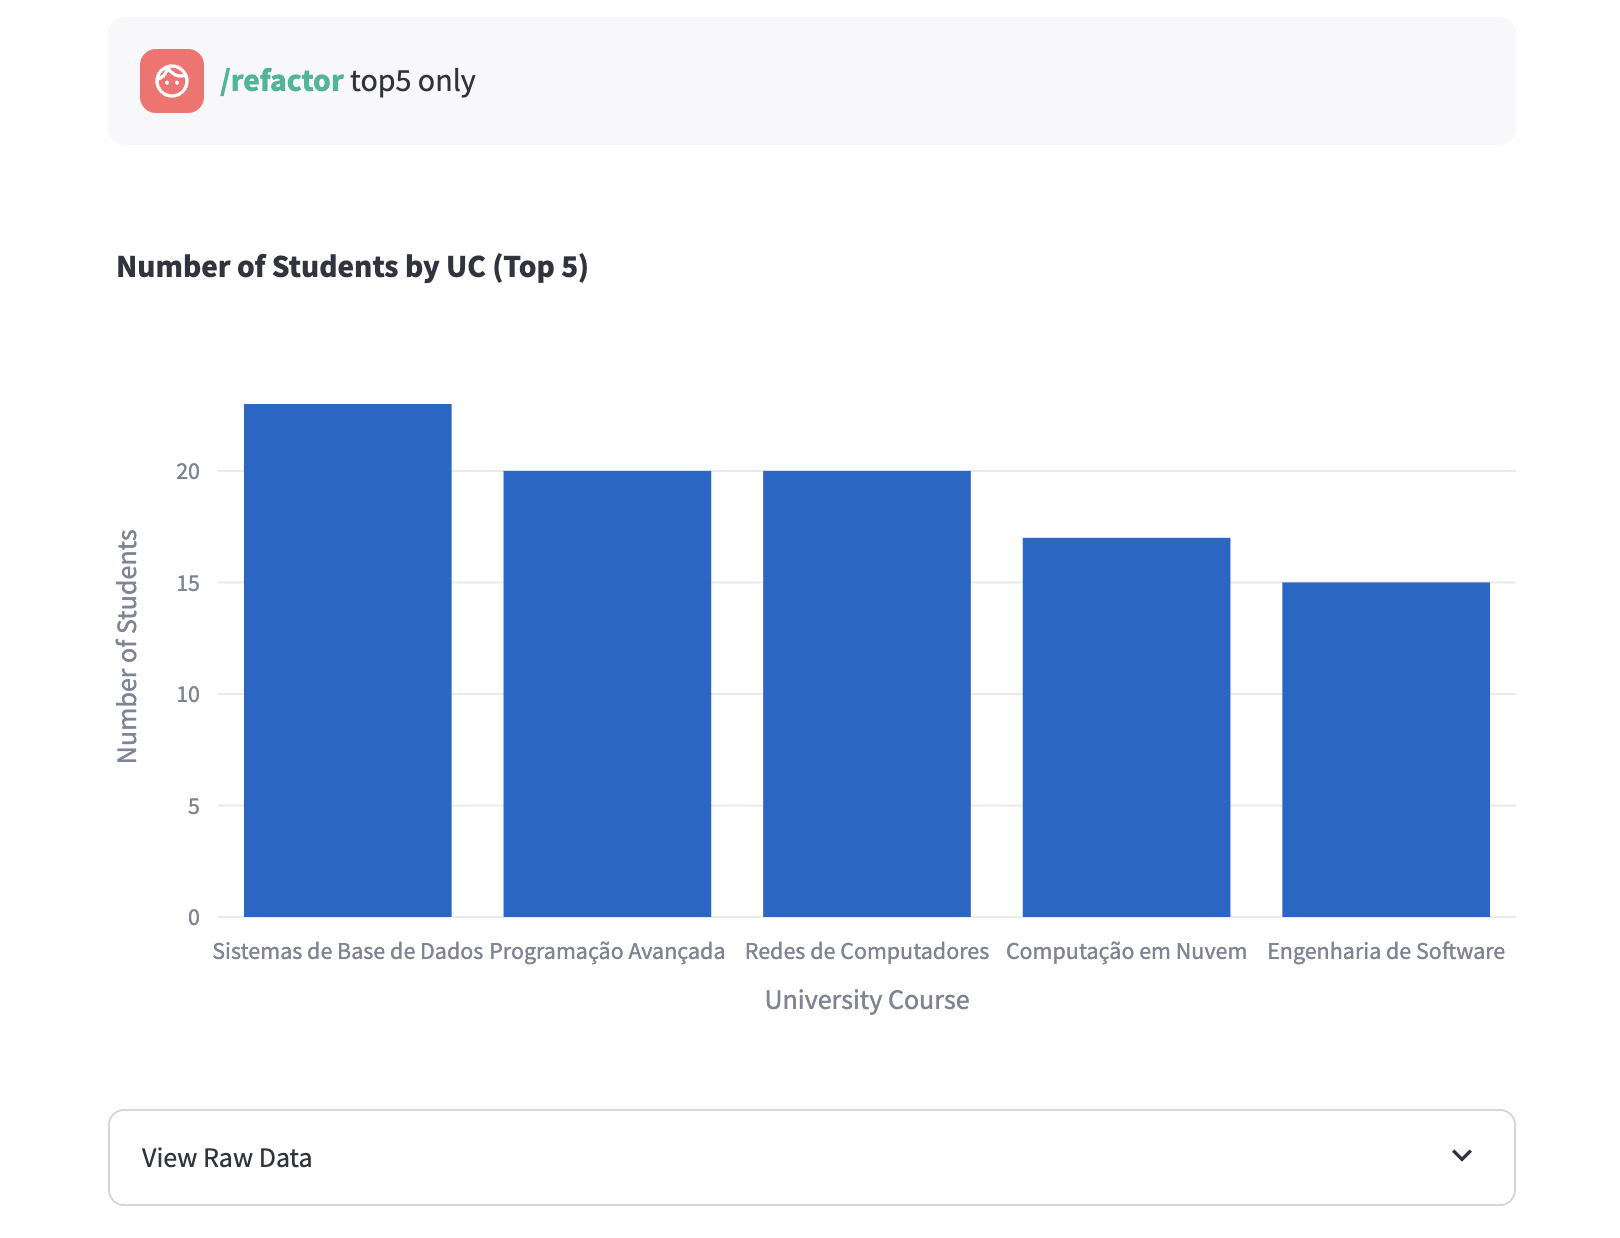
\includegraphics[width=\linewidth]{images/:refactor.png}
        \caption{Exemplo do comando /refactor}
        \label{fig:tables}
    \end{minipage}
\end{figure}

\hspace*{1em} Além das funcionalidades principais descritas anteriormente, foi adicionado ao programa um conjunto de comandos no mesmo estilo do \textbf{GitHub Copilot}, com o objetivo de auxiliar os utilizadores que possam ter dúvidas sobre os resultados gerados.  

Os comandos implementados são:  

\begin{itemize}
    \item \textbf{/sql} – Retorna a query SQL gerada a partir do prompt inserido pelo utilizador.
    \item \textbf{/tables} – Exibe a lista de tabelas disponíveis na base de dados, permitindo ao utilizador compreender melhor a estrutura dos dados.
    \item \textbf{/chart} – Apresenta o código Python utilizado para gerar o gráfico, facilitando a personalização e compreensão da visualização.
    \item \textbf{/explain} – Explica os resultados obtidos no DataFrame gerado a partir da query executada na base de dados, ajudando o utilizador a interpretar os dados retornados.
    \item \textbf{/refactor} – Permite modificar o último prompt inserido com novas informações.
    \item \textbf{/reset} – Elimina toda a conversa da interface em que estiver, permitindo recomeçar uma nova conversa sem histórico anterior.
    \item \textbf{/help} – Exibe a mensagem de ajuda com todos os comandos disponíveis.
\end{itemize}

 Estes comandos foram projetados para melhorar a experiência do utilizador, tornando a aplicação mais interativa e acessível. Com eles, o utilizador pode obter informações detalhadas sobre as consultas geradas, os dados disponíveis e a lógica por trás das respostas fornecidas pelo sistema. O comando **/reset**, em particular, facilita a reinicialização da conversa, garantindo um ambiente limpo para novas interações.  


\section{Testes}

Para avaliar o desempenho do modelo na conversão de linguagem natural em SQL, realizamos vários testes utilizando a base de dados previamente descrita. A seguir, explico os testes realizados, as consultas em linguagem natural fornecidas ao modelo e as respectivas consultas SQL geradas, a fim de verificar a precisão e a adequação dos resultados.

\subsection{Teste 1: Consulta sobre Alunos e Cursos}

O primeiro teste usa uma base de dados relacionada ao contexto acadêmico e contém informações sobre alunos, cursos e matrículas.

\begin{figure}[!ht]
    \centering
    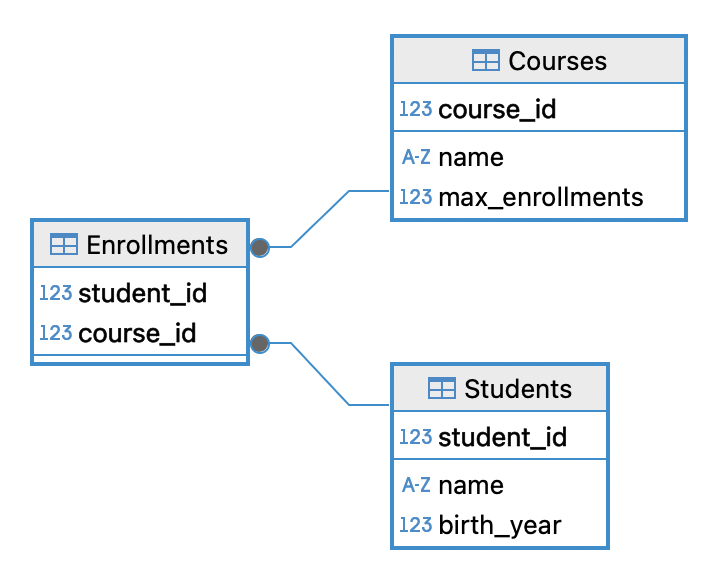
\includegraphics[width=0.5\linewidth]{images/schema1.png}
    \caption{Diagrama Entidade Relação}
    \label{fig:enter-label}
\end{figure}

A base dados é composta pelas seguintes tabelas:
\begin{itemize} 
    \item \textbf{Students} – Armazena informações sobre os alunos. 
    \item \textbf{Courses} – Armazena informações sobre os cursos oferecidos. 
    \item \textbf{Enrollments} – Armazena informações sobre as matrículas dos alunos nos cursos. 
\end{itemize}

Essas tabelas estão interligadas através dos campos \texttt{student\_id} e \texttt{course\_id}, permitindo consultas sobre alunos matriculados em cursos específicos ou informações sobre cursos com capacidade máxima de matrículas.

\subsubsection{Consulta: Listar todos os alunos matriculados em Sistemas de Base de Dados e nascidos em 2003}

A seguir, apresentamos os resultados da consulta solicitada. Mostramos as duas interfaces que geram os resultados: a primeira apresenta um relatório com os dados, e a segunda fornece uma explicação detalhada sobre o código SQL gerado.

\begin{figure}[ht]
    \centering
    \begin{minipage}{0.45\linewidth}
        \centering
        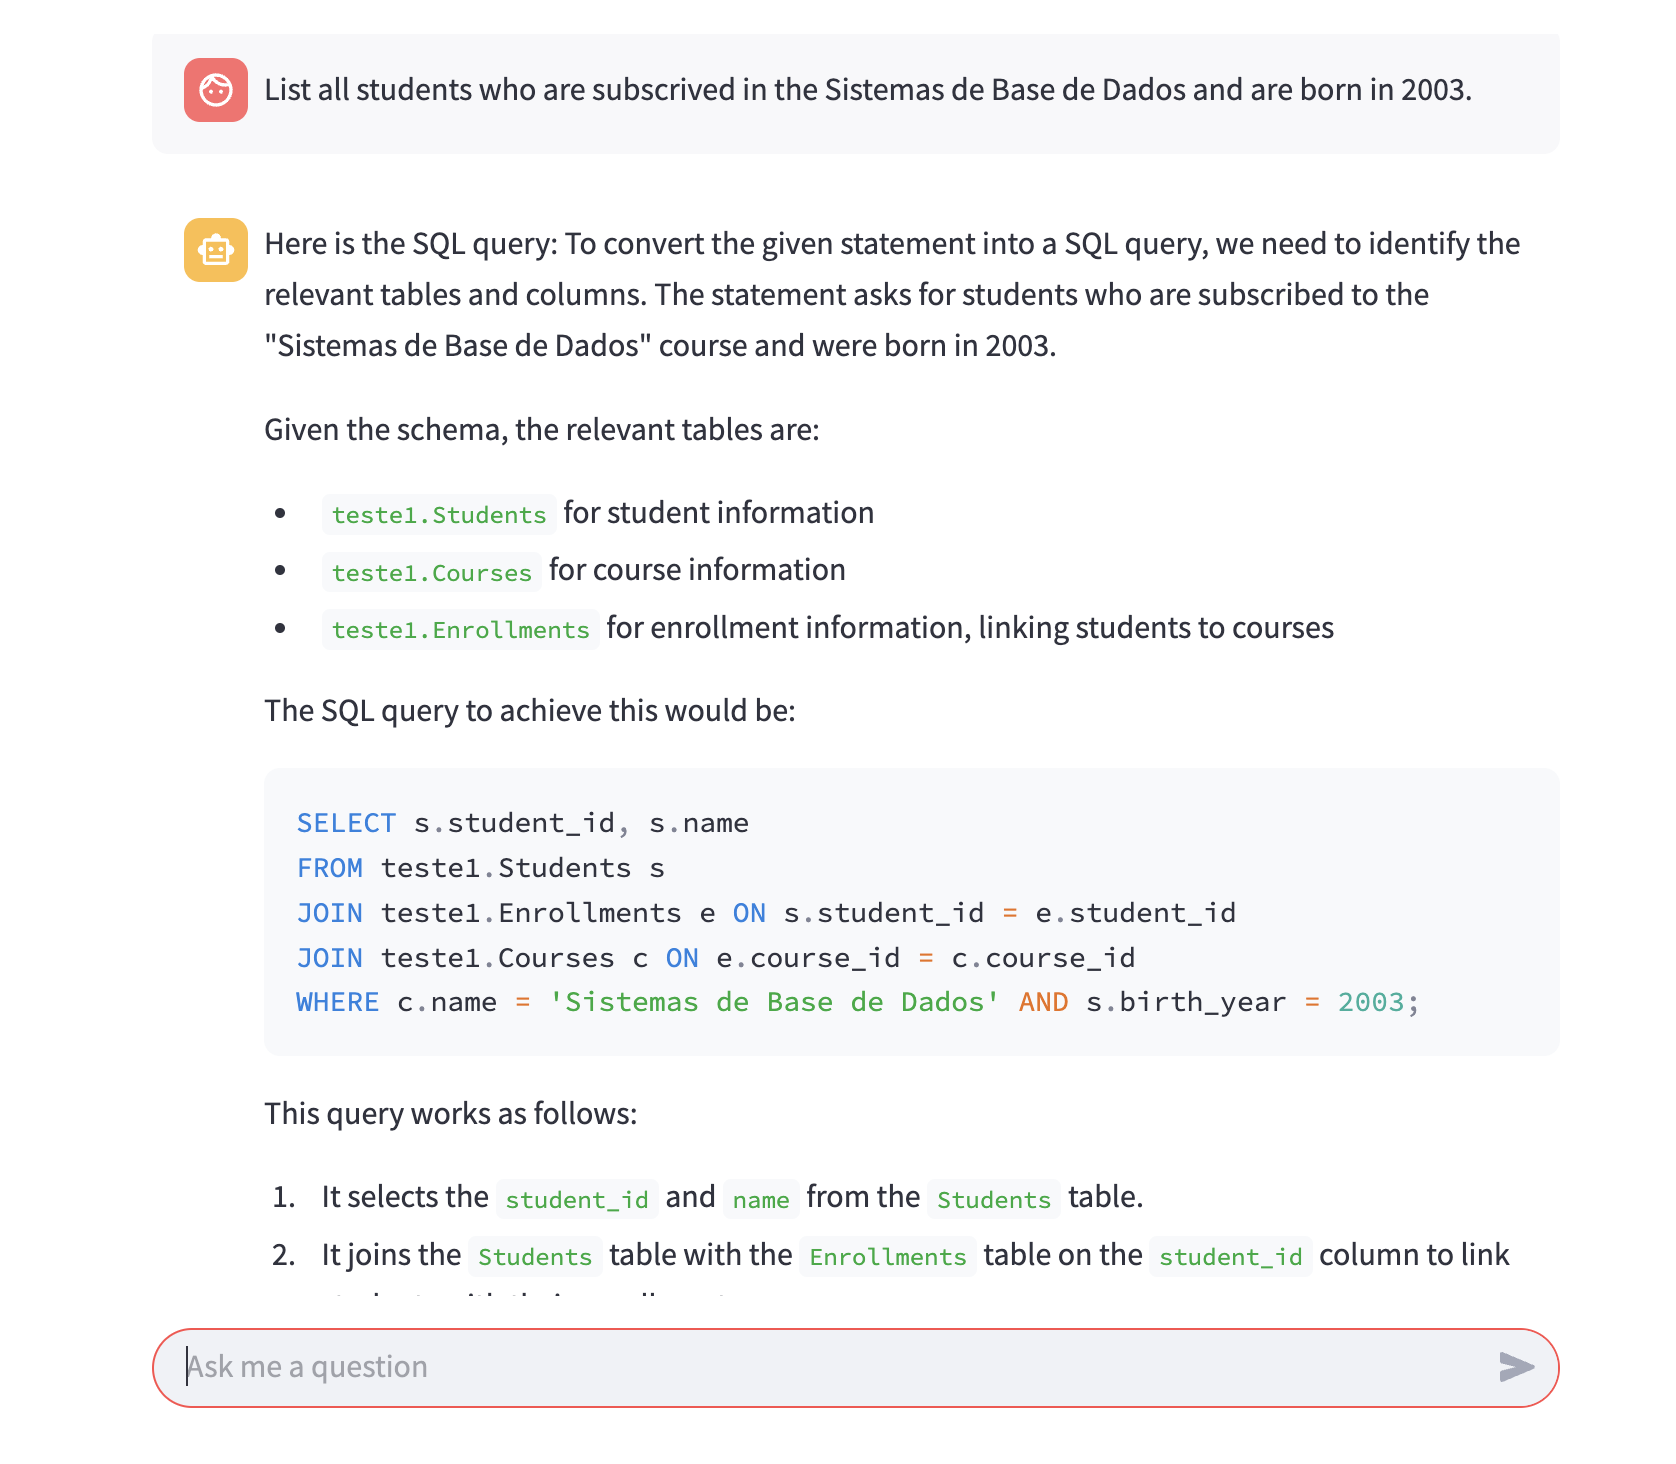
\includegraphics[width=\linewidth]{images/sql_generator1.png}
        \caption{Resposta gerada pelo SQL Generator}
        \label{fig:sql-generator}
    \end{minipage}
    \hspace{0.05\linewidth} % Espaço entre as imagens
    \begin{minipage}{0.45\linewidth}
        \centering
        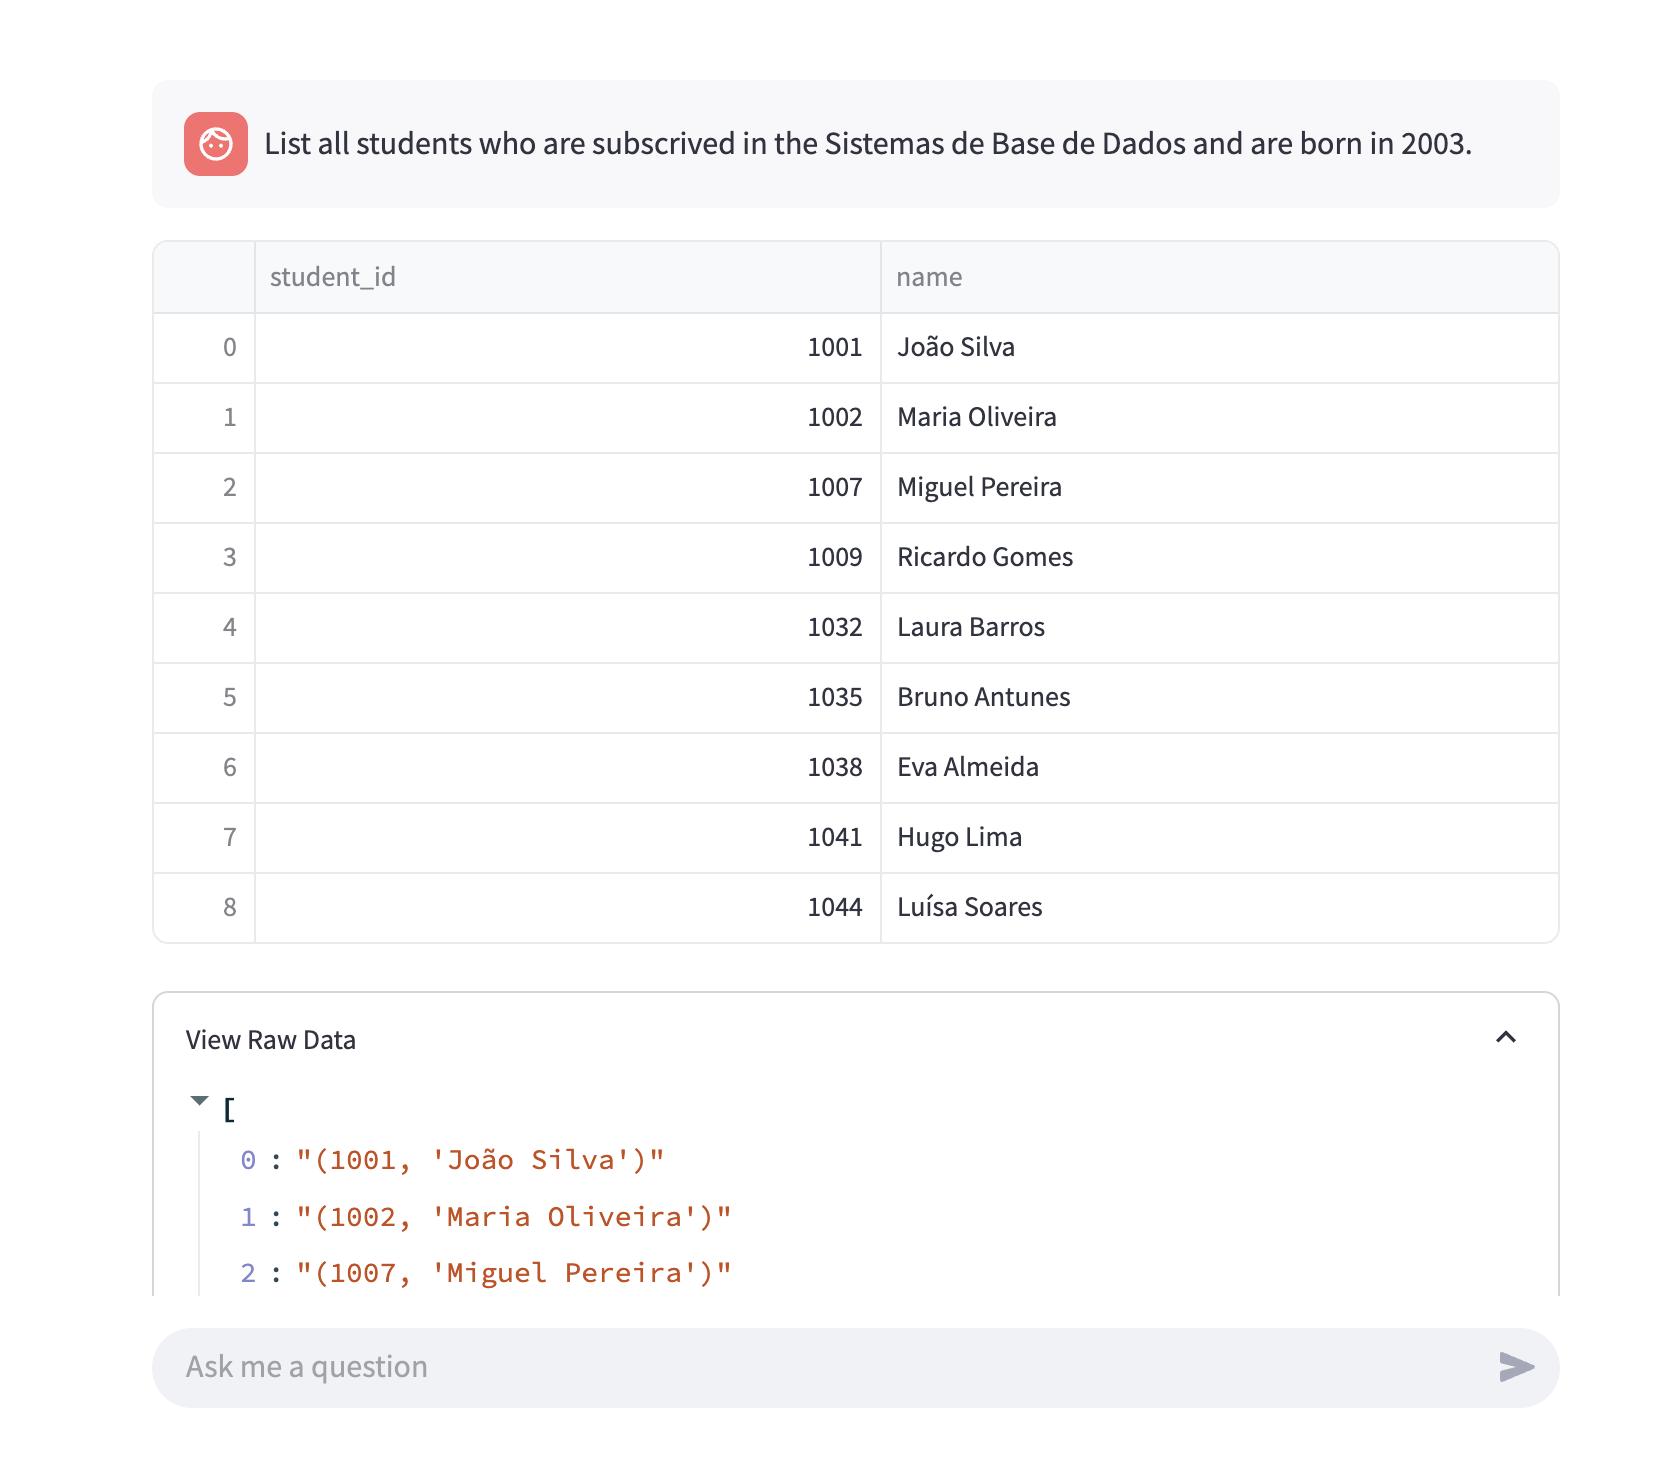
\includegraphics[width=\linewidth]{images/report_generator1.png}
        \caption{Resposta gerada pelo Report Generator}
        \label{fig:report-generator}
    \end{minipage}
\end{figure}

\paragraph{Explicação da Imagem \ref{fig:sql-generator} (SQL Generator):}

A primeira imagem (Figura \ref{fig:sql-generator}) mostra a consulta gerada pelo modelo.

\begin{verbatim}
SELECT s.student_id, s.name
FROM teste1.Students s
JOIN Enrollments e ON s.student_id = e.student_id
JOIN Courses c ON e.course_id = c.course_id
WHERE c.name = 'Sistemas de Base de Dados' AND S.birth_year = 2003;
\end{verbatim}

Além da consulta, a imagem apresenta uma explicação detalhada sobre o que cada parte da consulta faz, garantindo uma compreensão completa do processo de construção da query. A explicação fornece informações sobre a junção das tabelas \texttt{Students}, \texttt{Enrollments} e \texttt{Courses}, e a filtragem dos alunos de acordo com o curso e o ano de nascimento.

\paragraph{Explicação da Imagem  \ref{fig:report-generator} (Report Generator):}

A segunda imagem (Figura \ref{fig:report-generator}) mostra o resultado gerado pelo sistema Report Generator. Ao contrário da consulta SQL, que apresenta o código da query, o Report Generator exibe uma tabela com os alunos que atendem aos critérios especificados na consulta. A tabela contém os nomes dos alunos que estão matriculados no curso \texttt{Sistema de Base de dados} e que nasceram em \texttt{2003}, proporcionando uma visão direta e mais acessível dos resultados.

Ambas as abordagens geraram os resultados esperados, com a primeira focada na explicação da consulta SQL e a segunda fornecendo uma visualização prática e direta dos dados.

\subsubsection{Consulta: Lista a unidade curricular com maior numero de inscritos, os seus nomes e datas de nascimento.}

\begin{figure}[ht]
    \centering
    \begin{minipage}{0.3\linewidth}
        \centering
        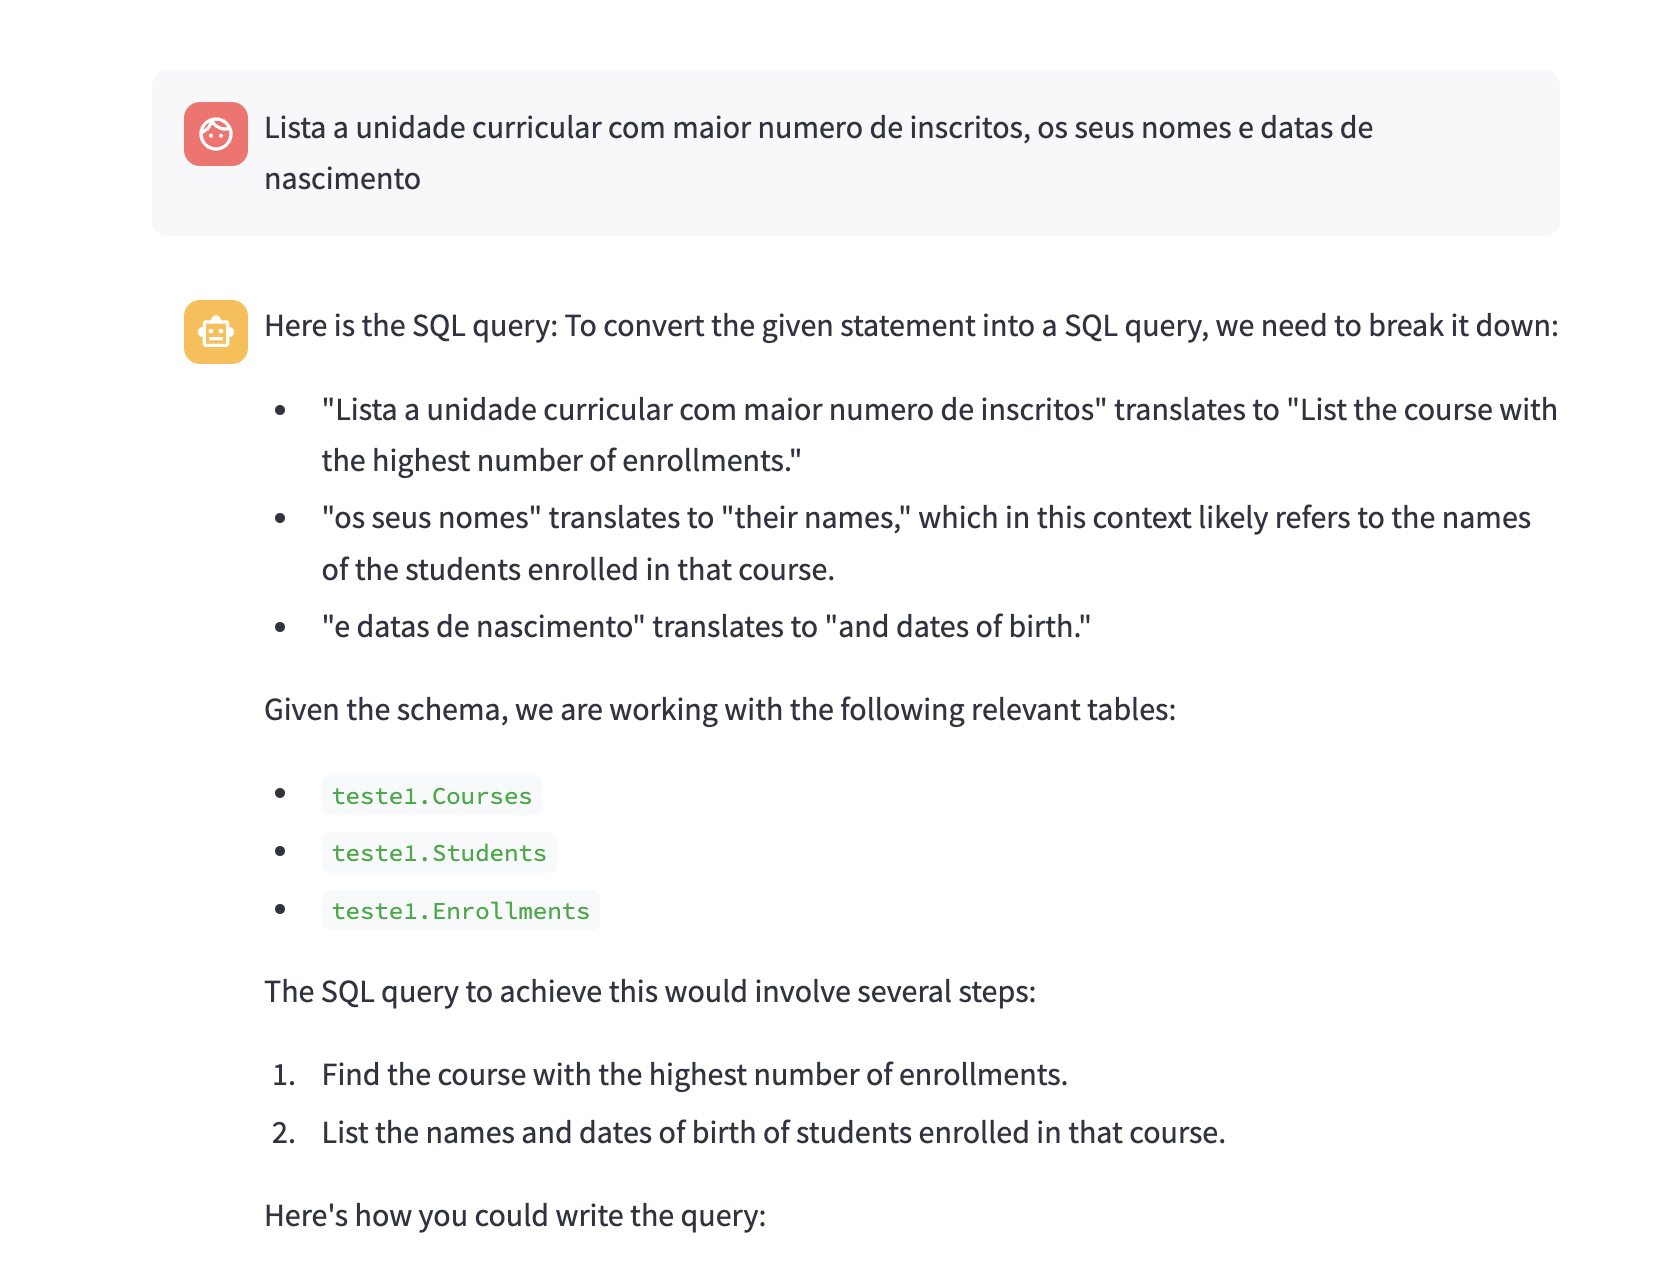
\includegraphics[width=\linewidth]{images/sql_generator2-1.png}
        \caption{Resposta gerada pelo SQL Generator}
        \label{fig:sql-generator2-1}
    \end{minipage}
    \hspace{0.01\linewidth} % Espaço entre as imagens
    \begin{minipage}{0.3\linewidth}
        \centering
        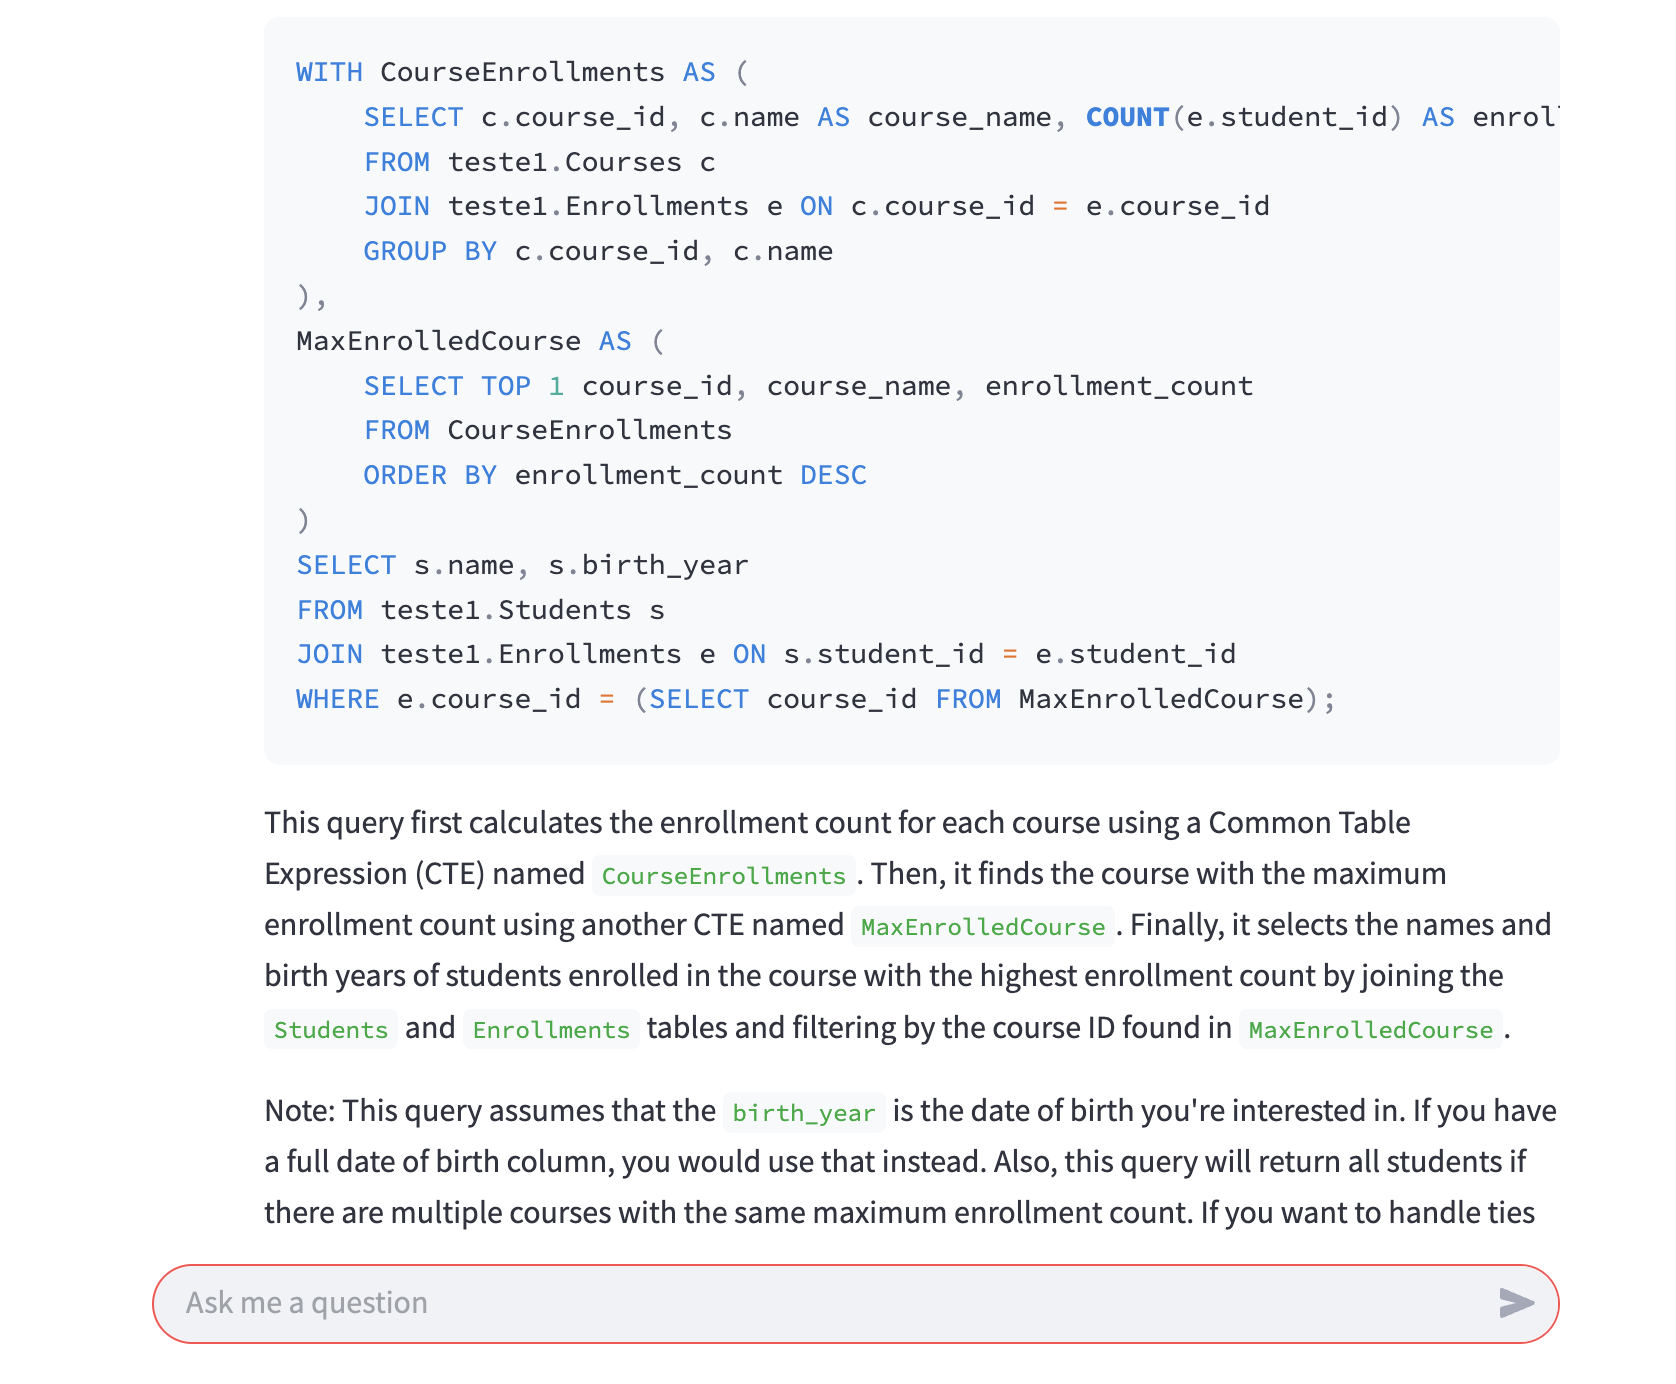
\includegraphics[width=\linewidth]{images/sql_generator2-2.png}
        \caption{Resposta gerada pelo SQL Generator}
        \label{fig:report-generator2-2}
    \end{minipage}
        \hspace{0.01\linewidth} % Espaço entre as imagens
    \begin{minipage}{0.3\linewidth}
        \centering
    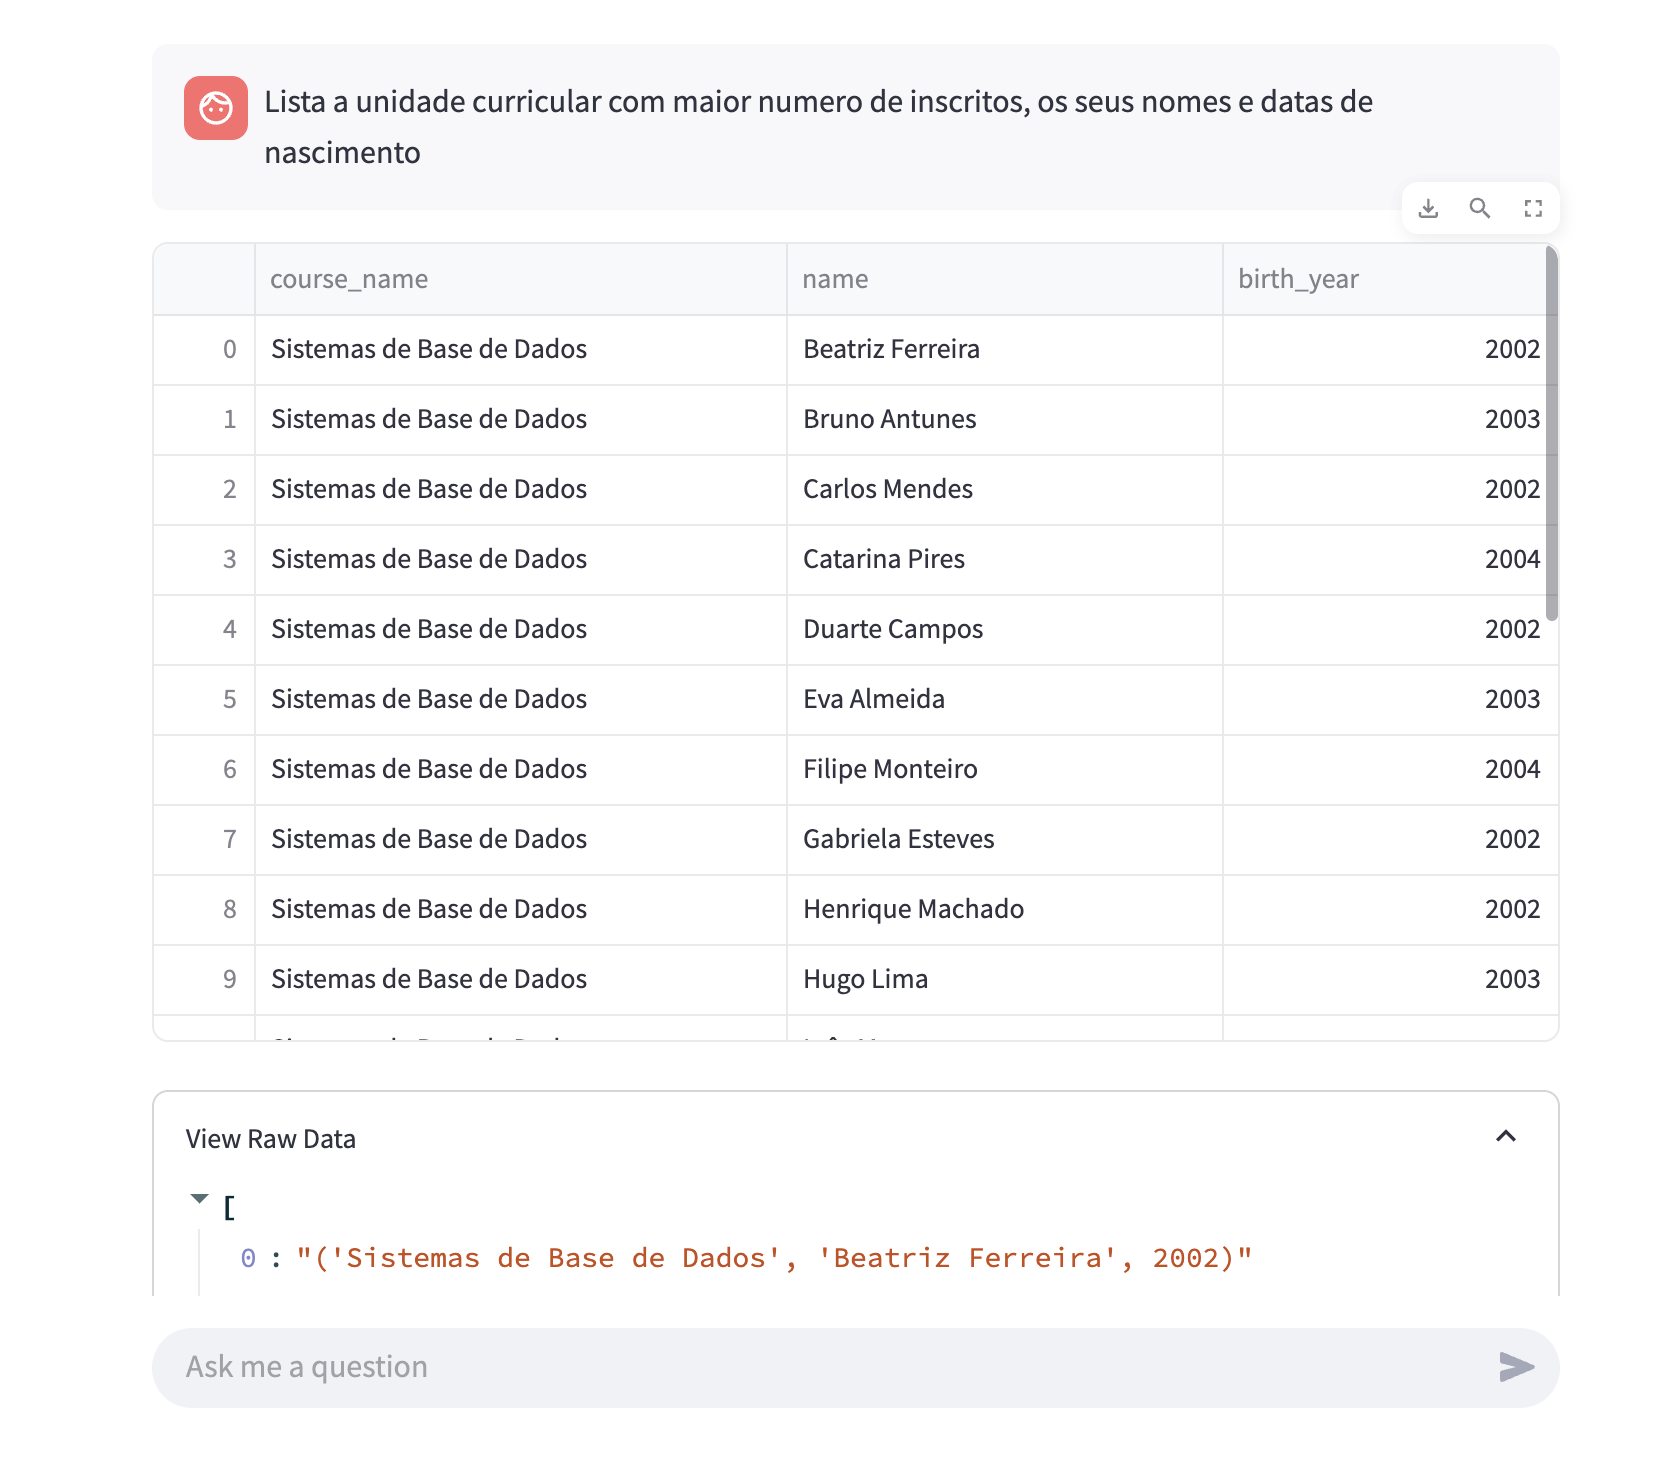
\includegraphics[width=\linewidth]{images/report_generator2.png}
    \caption{Resposta gerada pelo Report Generator}
    \label{fig:enter-label2}
    \end{minipage}
\end{figure}


\paragraph{Explicação da Imagem \ref{fig:sql-generator2-1} e Imagem \ref{fig:report-generator2-2} (SQL Generator):}

A primeira imagem (Figura \ref{fig:sql-generator}) mostra a consulta gerada pelo modelo. Além da consulta, a imagem apresenta uma explicação detalhada sobre a consulta, garantindo uma compreensão completa do processo de construção da query.

\paragraph{Explicação da Imagem  \ref{fig:enter-label2} (Report Generator):}

A imagem (Figura \ref{fig:enter-label2}) mostra o resultado gerado pelo sistema Report Generator. Ao contrário da consulta SQL, que apresenta o código da query, o Report Generator exibe uma tabela com os alunos que atendem aos critérios especificados na consulta. 

Novamente, ambas as abordagens geraram os resultados esperados, com a primeira focada na explicação da consulta SQL e a segunda fornecendo uma visualização prática e direta dos dados.


\subsubsection{Testes ao SQL Generator}


Após os testes realizados ao SQL Generator e ao Report Generator, realizei testes ao Chart Generator. Esta funcionalidade permite gerar gráficos com base na pergunta do utilizador, analisando a consulta realizada e apresentando a visualização correspondente.

\begin{figure}[ht]
    \centering
    \begin{minipage}{0.3\linewidth}
        \centering
        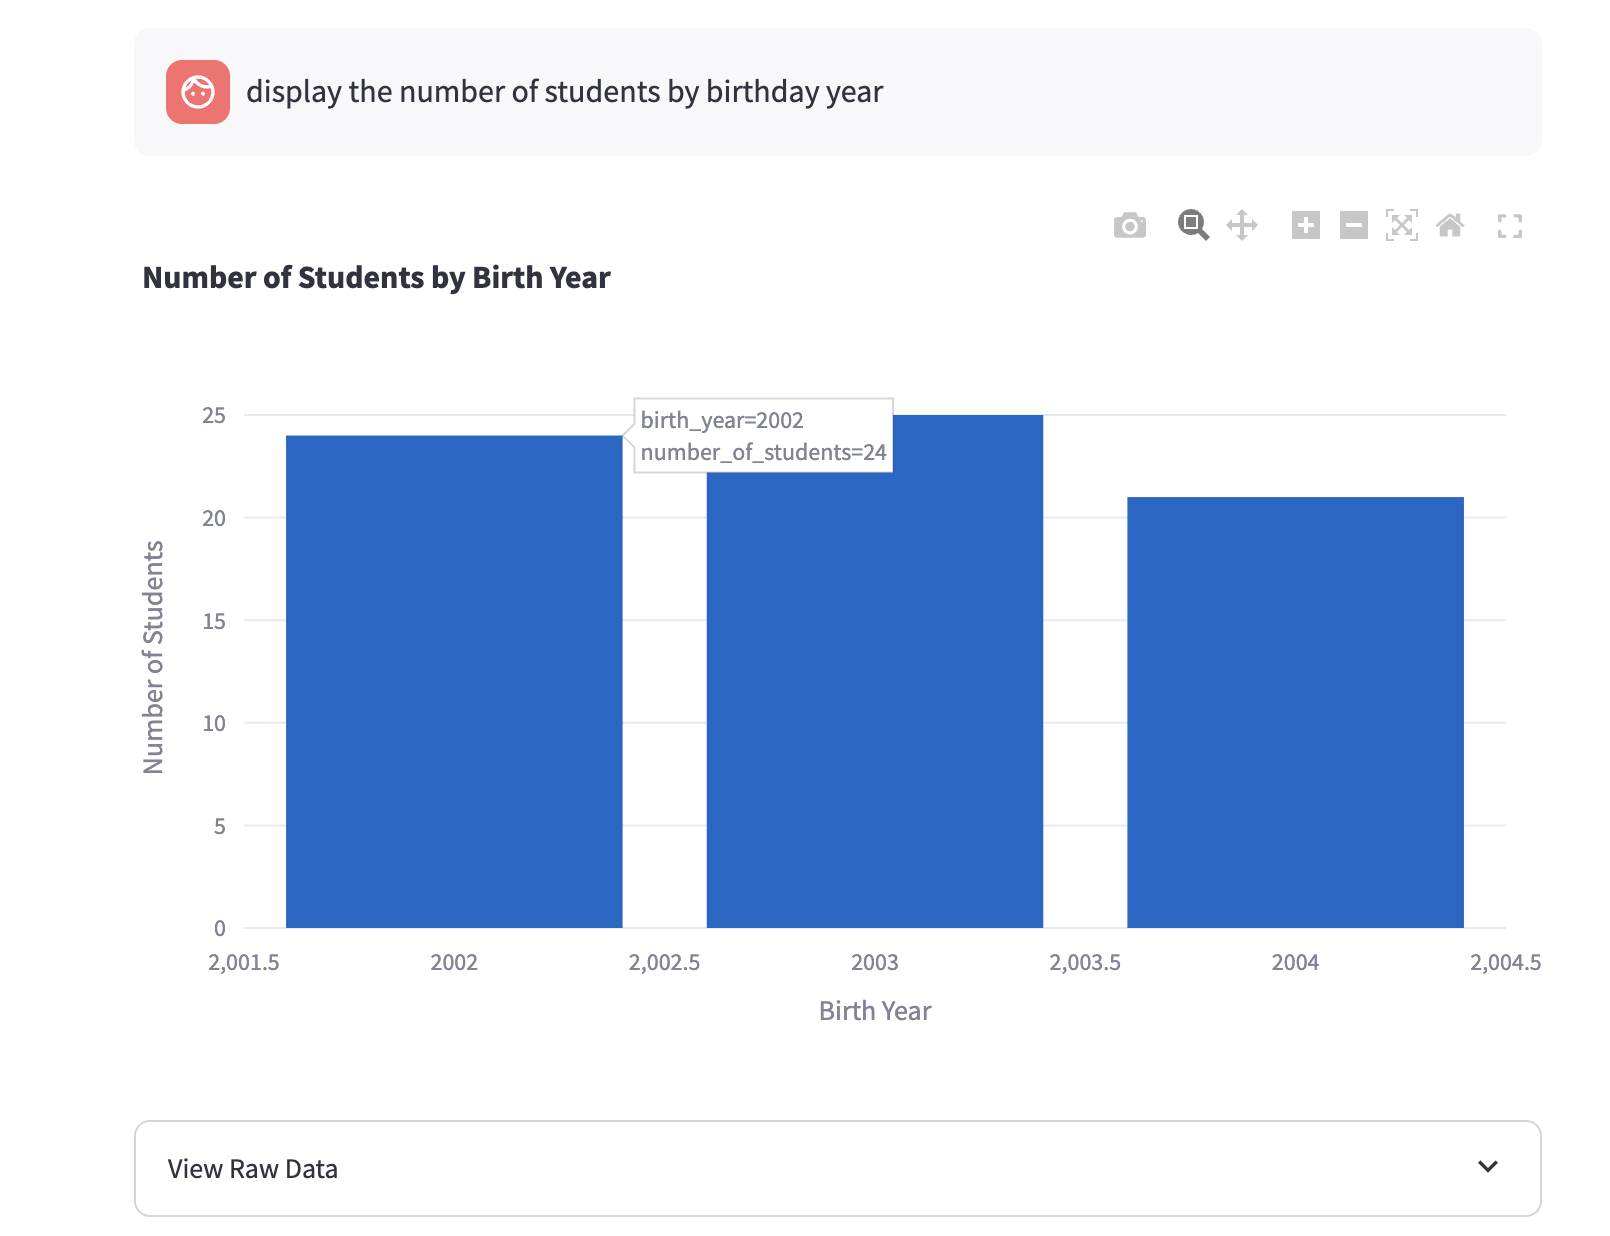
\includegraphics[width=\linewidth]
        {images/chart1.png}
        \caption{Resposta gerada pelo Chart Generator}
        \label{fig:chart1}
    \end{minipage}
    \hspace{0.01\linewidth} % Espaço entre as imagens
        \begin{minipage}{0.3\linewidth}
        \centering
        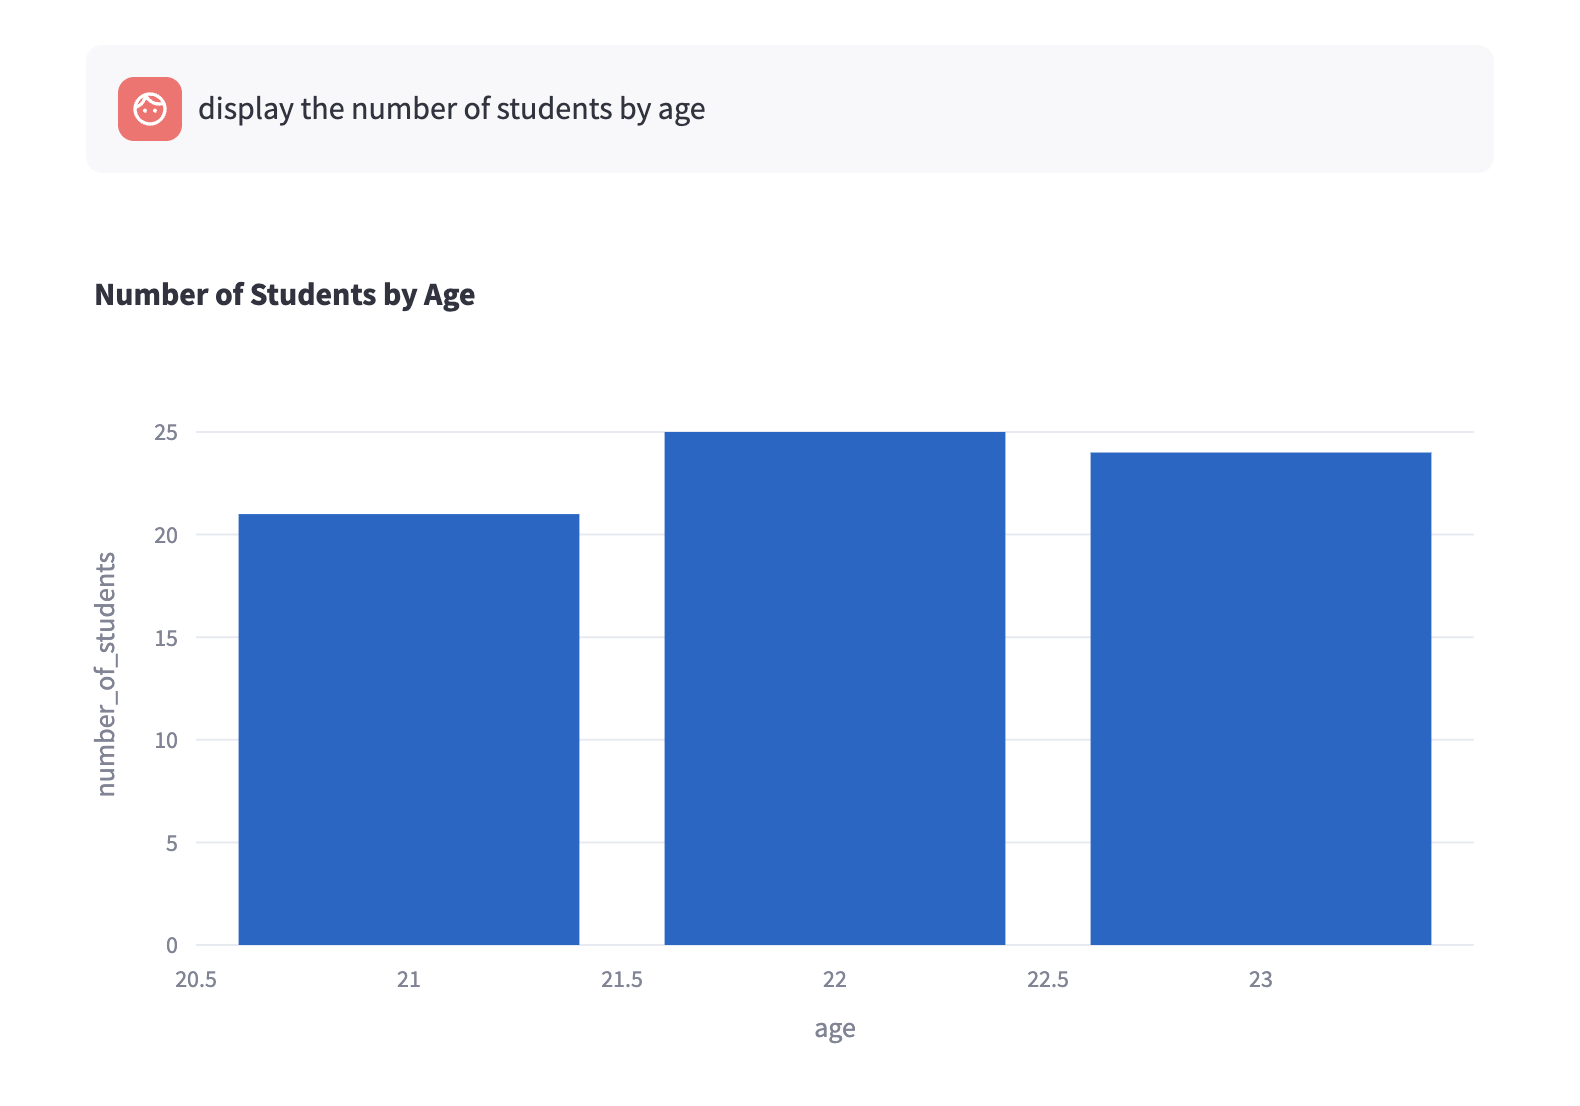
\includegraphics[width=\linewidth]
        {images/chart2.png}
        \caption{Resposta gerada pelo Chart Generator}
        \label{fig:chart2}
    \end{minipage}
    \hspace{0.01\linewidth} % Espaço entre as imagens
    \begin{minipage}{0.3\linewidth}
        \centering
        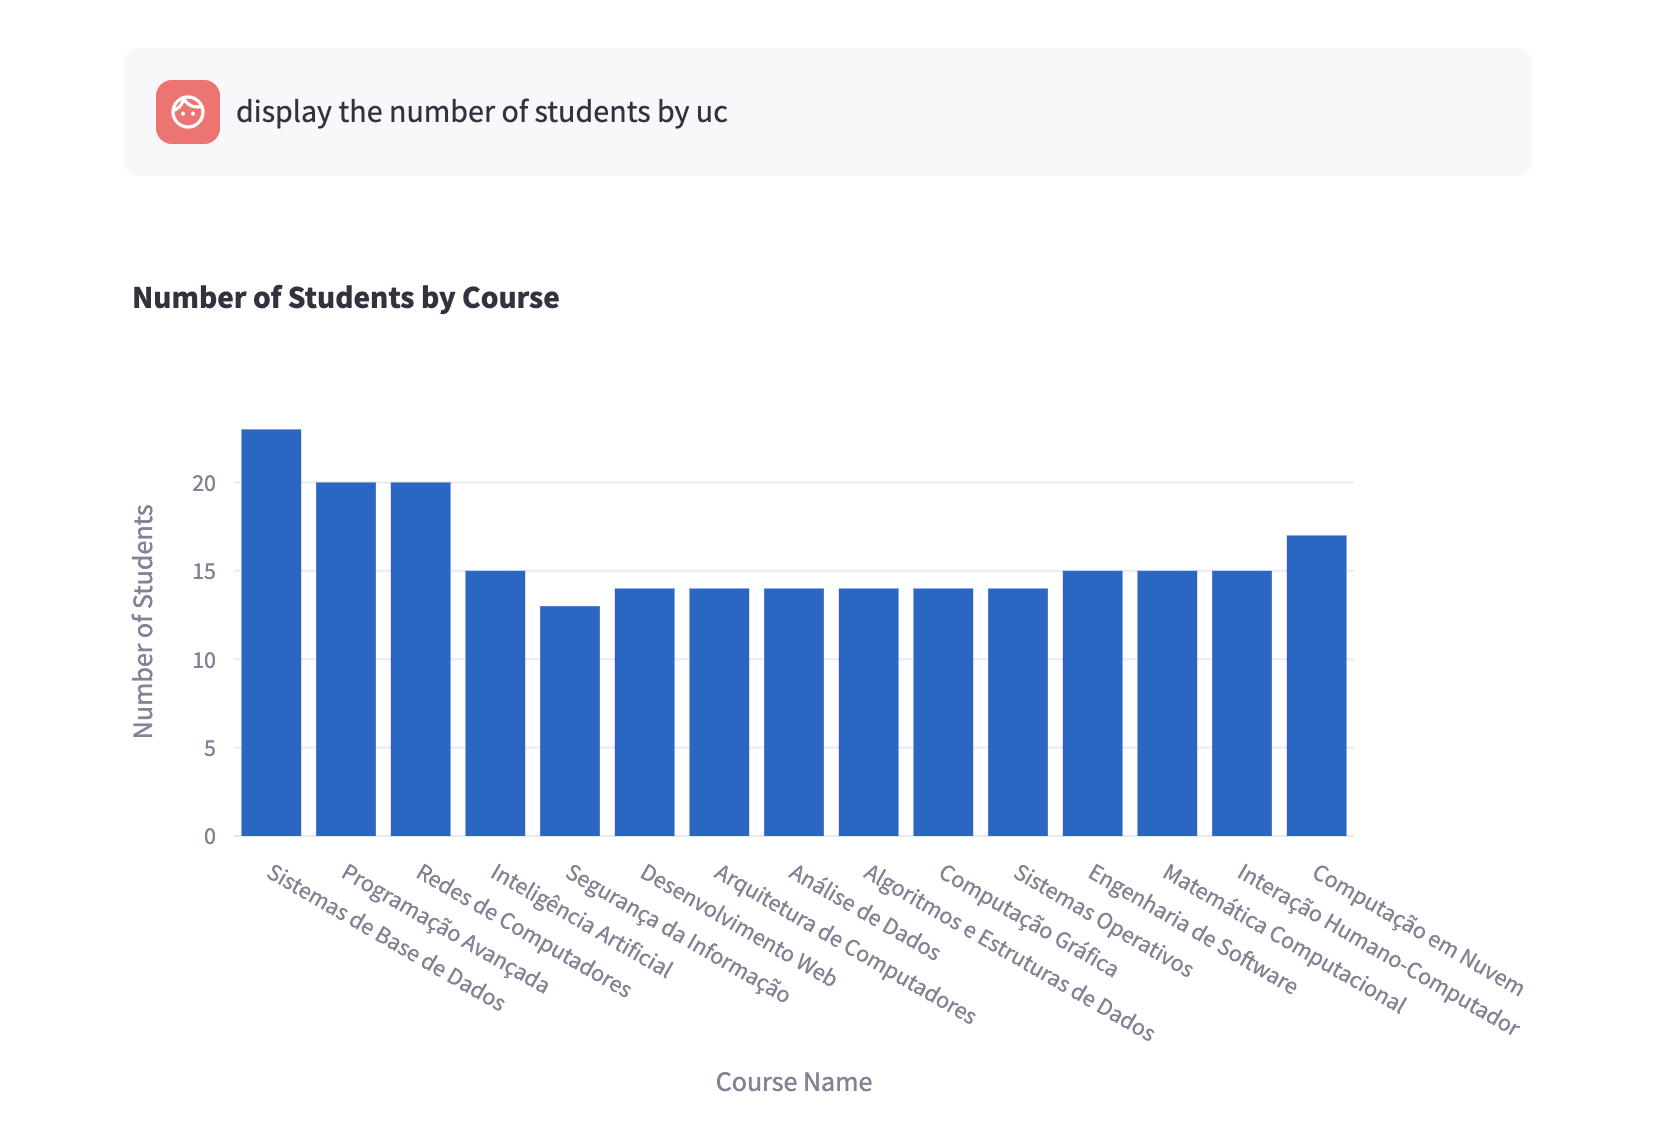
\includegraphics[width=\linewidth]
        {images/chart3.png}
        \caption{Resposta gerada pelo Chart Generator}
        \label{fig:chart3}
    \end{minipage}
\end{figure}

\paragraph{Imagem \ref{fig:chart1} Número de estudantes por ano de nascimento (Chart Generator):}

A primeira imagem (Figura \ref{fig:chart1}) apresenta o gráfico gerado pelo modelo, refletindo corretamente a distribuição do número de estudantes por ano de nascimento, conforme esperado.

\paragraph{Imagem \ref{fig:chart2} Número de estudantes por idade (Chart Generator):}

A Figura \ref{fig:chart2} exibe a distribuição do número de estudantes por idade, uma tarefa mais complicada uma vez que temos apenas na tabela a data de nascimento de cada indivíduo.

\paragraph{Imagem \ref{fig:chart3} Número de estudantes por Unidade Curricular (Chart Generator):}

Na Figura \ref{fig:chart3}, é apresentado um gráfico que mostra a distribuição do número de estudantes por Unidade Curricular (UC).

\subsection{Teste 2: AdventureWorks2012 Database}

\hspace*{1em} O segundo teste realizado recorre à base de dados AdventureWorks, amplamente utilizada para fins educativos e de prática com SQL. Esta base de dados simula o funcionamento de uma empresa fictícia de fabrico e venda de bicicletas, disponibilizando um conjunto rico de tabelas relacionadas com clientes, encomendas, produtos, funcionários, entre outras.

\begin{figure}[ht]
    \centering
    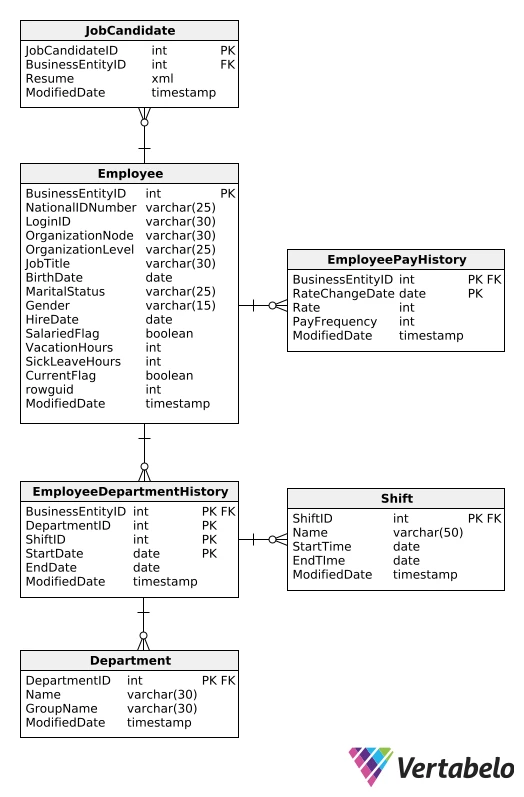
\includegraphics[width=0.25\linewidth]{AdvDiagram.png}
    \caption{Diagrama Entidade Relação Adventure Works}
    \label{fig:diaAdv}
\end{figure}

Para a elaboração deste teste, foram utilizadas perguntas disponíveis no seguinte recurso online, \textbf{AdventureWorks SQL Questions – LearnSQL.com \cite{learnsql2022}}


\subsubsection{Questões Utilizadas}

\hspace*{1em} As perguntas utilizadas neste teste foram extraídas do recurso online \textit{AdventureWorks SQL Questions – LearnSQL.com \cite{learnsql2022}}, abrangendo diferentes níveis de complexidade (Fácil, Médio e Difícil). Estas questões centram-se maioritariamente na área de Recursos Humanos (Figura~\ref{fig:diaAdv}) e permitiram avaliar diversas competências em SQL. Esta variedade permitiu testar a capacidade do modelo na geração de consultas SQL a partir da estrutura dos dados fornecida, possibilitando ainda a comparação entre os resultados obtidos pelas queries geradas automaticamente e as soluções disponibilizadas pelo site de origem. Abaixo apresenta-se a lista completa de perguntas:

\begin{enumerate}
    \item Selecionar o cargo (job title) de todos os funcionários do sexo masculino que não são casados.
    \item Selecionar o \texttt{BusinessEntityID}, a taxa (\texttt{Rate}) e a data de alteração da taxa (\texttt{RateChangeDate}) para todos os funcionários cuja taxa de pagamento tenha sido, em algum momento, igual ou superior a 50.
    \item Selecionar o \texttt{BusinessEntityID}, o \texttt{DepartmentID} e a data de início (\texttt{StartDate}) para cada funcionário que tenha começado a trabalhar em qualquer departamento durante o ano de 2008.
    \item Selecionar os IDs, nomes e nomes dos grupos dos departamentos cujo nome começa por ``Prod'' OU cujo nome do grupo termina em ``ring''.
    \item Selecionar os nomes dos departamentos que pertencem ao grupo ``Research and Development'' ou ao grupo ``Manufacturing''.
    \item Selecionar os IDs dos funcionários juntamente com todos os nomes dos departamentos onde trabalharam em qualquer momento.
    \item Selecionar o ID e o cargo (job title) do funcionário, juntamente com as datas de mudança de departamento (\texttt{StartDate}), apenas para funcionárias do sexo feminino.
    \item Selecionar os cargos (job titles) e os respetivos nomes dos departamentos, de forma a identificar todos os cargos que foram alguma vez utilizados em cada departamento. Não incluir duplicados.
    \item Selecionar os nomes distintos de departamentos e turnos (shifts) em que trabalham os funcionários. Renomear as colunas para \texttt{DepartmentName} e \texttt{ShiftName}.
    \item Selecionar os IDs dos funcionários, nomes dos departamentos e nomes dos turnos, incluindo apenas funcionários contratados após 01-01-2010 e que trabalham em departamentos pertencentes aos grupos ``Manufacturing'' ou ``Quality Assurance''.
    \item Selecionar o número mínimo e máximo de horas de baixa médica (\texttt{sick leave}) tiradas pelos funcionários.
    \item Selecionar os cargos e o número médio de horas de férias (\texttt{vacation hours}) por cargo.
    \item Selecionar o sexo dos funcionários e a contagem de funcionários por cada género.
    \item Contar o número de departamentos em cada grupo de departamentos. Listar apenas os grupos de departamentos que têm mais de dois departamentos.
    \item Selecionar os nomes dos departamentos e a soma de horas de baixa médica tiradas pelos funcionários que atualmente trabalham em cada departamento. Renomear esta coluna para \texttt{SumSickLeaveHours}.
    \item Selecionar os IDs dos funcionários e as suas taxas de pagamento atuais.
    \item Selecionar os valores mínimo, médio e máximo das taxas de pagamento atuais dos funcionários.
    \item Selecionar os IDs dos funcionários que tiraram mais de 60 horas de férias ou mais de 60 horas de baixa médica.
    \item Selecionar os IDs dos funcionários que têm os cargos ``Sales Representative'' ou ``Tool Designer'' e que tenham trabalhado (ou estejam a trabalhar) nos departamentos de Vendas (\texttt{Sales}) ou Marketing. Ordenar por valor, do mais alto para o mais baixo.
    \item Selecionar os IDs, cargos e nomes dos departamentos dos funcionários associados às funções de ``Sales Representative'' ou ``Marketing Manager''.
\end{enumerate}

\subsubsection{Resultados Obtidos}

\hspace*{1em} Para realizar a comparação, comecei por gerar as 20 consultas SQL utilizando o meu algoritmo. Cada query gerada foi então comparada com as consultas de referência fornecidas pelo site, que representavam as respostas esperadas. O objetivo era verificar a precisão e a eficácia das consultas geradas, avaliando se os resultados estavam de acordo com os dados esperados. As consultas foram avaliadas de acordo com os seguintes critérios:

\begin{itemize}
    \item Equal: Quando os resultados retornados correspondiam exatamente aos dados esperados, independentemente de variações em nomes de colunas ou ordenações.
    \item Correct+: Quando a query retornava todos os dados esperados, com a adição de colunas extras que não comprometeram a integridade dos dados.
    \item Correct-: Quando a consulta retornava dados corretos, com uma correspondência superior a 90\% dos dados esperados, mas com pequenas variações na estrutura da resposta.
    \item Incorrect: Quando a consulta retornava dados completamente diferentes dos esperados, com falhas significativas que indicavam uma abordagem errada na construção da query, resultando em um conjunto de dados que não correspondia à intenção da pergunta original.
    \item No Results: Quando nenhuma das query retornava nenhum dado, o que indicava um erro no proprio resultado de comparação.
\end{itemize}
Após a execução e comparação das 20 queries, os seguintes resultados foram observados:

\begin{itemize}
    \item 15 queries (75\%) foram classificadas como "Equal", o que significa que os dados retornados coincidiam exatamente com os dados esperados. Embora em alguns casos houvesse variações nos nomes das colunas ou na ordem delas, as informações retornadas eram consistentes com o que se esperava.
    \item 1 query (Q2) recebeu a classificação "Correct+", além de retornar todos os dados esperados, incluiu colunas adicionais que enriqueceram a resposta, sem comprometer a integridade dos dados principais.
    \item 1 query (Q6) foi classificada como "Correct-", indicando que os dados estavam corretos em +90\%, mas houve uma pequena diferença em relação ao esperado. Isto pode ter ocorrido devido a uma exceção ausente ou uma comparação incorreta, resultando em uma ligeira discrepância nos resultados.
    \item 2 queries (Q3 e Q10) resultaram em "No Results", ou seja, não retornaram dados. Esse resultado pode ser atribuído a filtros muito restritivos ou a aplicação de intervalos de datas muito específicos, que não correspondiam aos dados presentes na base de dados.
\end{itemize}

Os resultados demonstram que o algoritmo foi eficaz em gerar as consultas SQL e que a maioria das queries geradas produziu resultados idênticos aos esperados. A alta taxa de acerto (75\%) sugere uma sólida compreensão das técnicas de SQL, especialmente no uso de JOIN, filtros e agregações.
As discrepâncias observadas em algumas consultas podem ser atribuídas a diferenças na forma de apresentação dos dados ou a filtros que não encontraram correspondência nos dados da base de dados.

\subsection{Teste 3: TPC-H Database}

\hspace*{1em} O terceiro teste realizado utilizou a base de dados TPC-H, um benchmark amplamente utilizado para avaliar o desempenho de sistemas de processamento de consultas complexas. A TPC-H simula um ambiente de negócios de uma empresa de vendas de produtos e serviços, com um conjunto de dados que abrange várias tabelas relacionadas a vendas, clientes, linha de pedidos, entre outros.


\begin{figure}
    \centering
    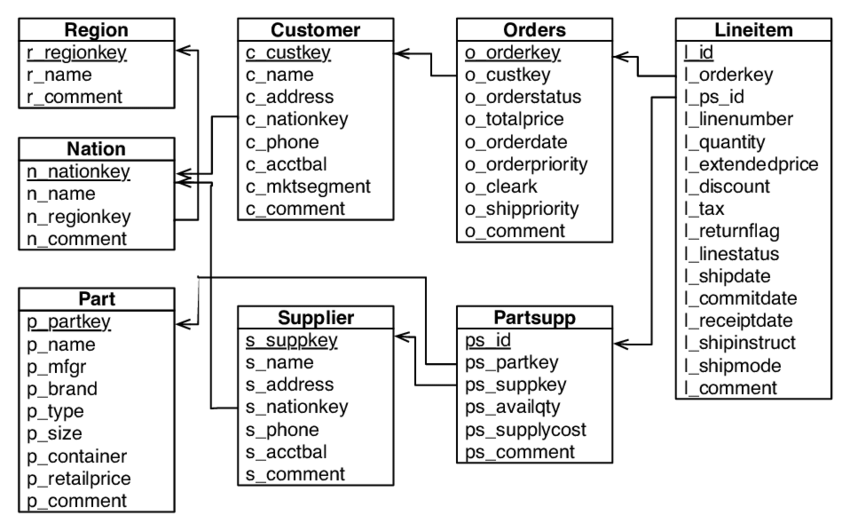
\includegraphics[width=0.5\linewidth]{image.png}
    \caption{TPC-H Diagrama Entidade Relação}
    \label{fig:enter-label}
\end{figure}

Para a elaboração deste teste, foram utilizadas questões disponíveis no recurso online \textbf{TPC-H Benchmark Queries – TPC.org \cite{tpc-h}}. Essas questões foram formuladas com o objetivo de avaliar o desempenho das consultas em diferentes áreas de processamento de dados, incluindo operações de agregação, join e filtragem, simulando cenários complexos de consultas analíticas.

\subsubsection{Questões Utilizadas}

\hspace*{1em} As questões utilizadas neste teste foram extraídas do benchmark TPC-H, abordando diversas áreas de análise de dados. Essas questões envolvem desde consultas simples de agregação até consultas complexas que utilizam múltiplos joins e agrupamentos. As consultas foram utilizadas para avaliar a eficácia do modelo na geração de queries SQL que correspondessem aos resultados esperados. Abaixo apresenta-se uma lista parcial de perguntas:

\begin{enumerate} 
    \item Selecionar o total de vendas por cada cliente, ordenado pela maior quantidade de vendas. 
    \item Calcular a média e o desvio padrão das vendas por segmento de mercado. 
    \item Identificar os produtos que tiveram mais de 50 vendas no último trimestre. \item Calcular a receita total por ano e por região. 
    \item Identificar os 10 produtos mais vendidos durante o ano, com base no total de unidades vendidas. 
    \item Calcular o valor médio das transações para cada ano. 
    \item Identificar os 5 fornecedores com as maiores vendas no último ano. 
    \item Calcular o valor total das vendas de produtos em regiões específicas. 
    \item Identificar os 10 clientes que mais gastaram com a compra de produtos no último trimestre. 
    \item Calcular a variação anual nas vendas por produto. 
    \item Calcular a soma das vendas de cada produto por trimestre. 
    \item Obter a média de vendas por categoria de produto para cada ano. 
    \item Calcular o valor total de vendas para os produtos que foram vendidos por mais de um fornecedor. 
    \item Selecionar a receita total por ano e por categoria de produto. 
    \item Calcular o número de pedidos realizados por cliente e a média de itens por pedido. 
    \item Obter os produtos que representam mais de 5\% da receita total por categoria. 
    \item Calcular a quantidade de pedidos realizados por cada cliente durante o ano. \item Identificar as regiões com a maior receita total no último ano. 
    \item Calcular o total de vendas por região e por categoria de produto. 
    \item Calcular o número de transações por cliente em cada região. 
\end{enumerate}

\subsubsection{Resultados Obtidos}

\hspace*{1em} Para a execução do teste, as consultas SQL foram geradas automaticamente utilizando o algoritmo proposto. Cada query gerada foi comparada com as consultas de referência fornecidas pelo site, que continham as respostas esperadas. O objetivo era verificar a precisão e a eficácia das consultas geradas, avaliando se os resultados estavam de acordo com os dados fornecidos na base TPC-H.

Após a execução e comparação das 22 queries, os seguintes resultados foram observados:

\begin{itemize} 
\item 17 queries (77\%) foram classificadas como "Equal", indicando que os dados retornados coincidiram exatamente com os dados esperados. Embora houvesse algumas variações nos nomes das colunas ou na ordem delas, as informações retornadas foram consistentes com o que se esperava. 
\item 3 queries (Q3, Q7 e Q21) receberam a classificação "Correct-", pois os dados retornados estavam corretos, com mais de 90\% de correspondência com os resultados esperados, mas com pequenas diferenças. 
\item 2 queries (Q9 e Q20) foram classificadas como "Incorrect", ou seja, retornaram dados completamente diferentes do esperado, indicando algumas falhas, provavelmente na agregação. \end{itemize}

Estes resultados demonstram que o algoritmo foi eficaz na geração das consultas SQL e que a maioria das queries geradas produziu resultados idênticos aos esperados. A elevada taxa de acerto (77\%) sugere novamente uma boa compreensão da estrutura da base de dados TPC-H e das operações SQL necessárias para recuperar os dados de forma eficiente. As discrepâncias observadas em algumas consultas podem ser atribuídas a pequenas variações na forma de apresentação dos dados ou a diferenças na interpretação dos requisitos das perguntas.

\begin{figure}[ht]
    \centering
    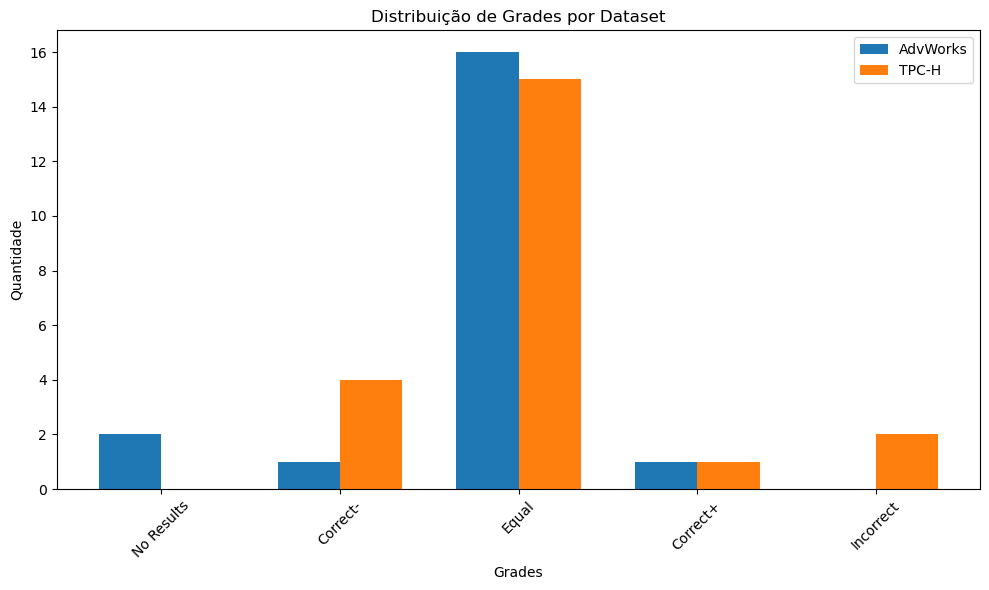
\includegraphics[width=0.75\linewidth]{comparResults.png}
    \caption{Gráfico de acerto dos testes}
    \label{fig:enter-label}
\end{figure}

\section{Conclusões}

Nos dias de hoje, a inteligência artificial (IA) tem revolucionado o mercado de diversas formas, trazendo tanto benefícios quanto desafios. Em áreas como a análise de dados e a manipulação de bases de dados, a IA tem se mostrado uma poderosa aliadas, ao permitir que pessoas sem formação técnica interajam de maneira simples e intuitiva com grandes volumes de dados, a IA está a facilitar a tomada de decisões, automatizando processos e, principalmente, abrindo portas para que mais pessoas possam tirar proveito do vasto potencial das bases de dados.

No entanto, a aplicação de IA nesse campo não está isenta de dificuldades. Um dos maiores desafios é garantir que os modelos consigam traduzir perguntas em linguagem natural para consultas SQL precisas, especialmente em cenários mais complexos que envolvem múltiplas tabelas e operações avançadas. O caminho até encontrar a solução ideal para o meu projeto foi marcado por vários testes e tentativas de diferentes modelos, até finalmente encontrar uma solução robusta com o Llama-3.3-70b-versatile da Groq. Este modelo mostrou-se capaz de lidar de forma eficiente com as complexidades das consultas SQL, oferecendo respostas mais precisas e adequadas às perguntas feitas.

O objetivo principal deste projeto foi criar uma ferramenta acessível que permitisse a qualquer pessoa, mesmo sem conhecimentos técnicos em bases de dados, gerar consultas SQL a partir de perguntas em linguagem natural. Ao longo do desenvolvimento, foram implementados diversos testes para garantir que a aplicação não apenas gerasse consultas corretas, mas também fosse capaz de recuperar os dados de forma eficaz e apresentar gráficos de maneira precisa. Para melhorar ainda mais a experiência do utilizador, a aplicação inclui funcionalidades adicionais que ajudam na navegação e no entendimento dos dados, como já falado anteriormente.

Estas funcionalidades contribuem para uma experiência mais fluida e intuitiva, permitindo aos utilizadores não apenas obter as respostas que procuram, mas também entender como essas respostas são geradas e apresentadas. Assim, a IA no contexto deste projeto não apenas cumpre a função de facilitar a geração de queries, mas também de educar e apoiar os utilizadores no processo da análise de dados.

Em suma, este projeto é um exemplo de como a inteligência artificial pode ser aplicada para resolver problemas reais e complexos, tornando ferramentas avançadas de análise de dados acessíveis para todos.

\bibliography{refs}
\bibliographystyle{IEEEtran}

\end{document}
